\documentclass[]{book}
\usepackage{lmodern}
\usepackage{amssymb,amsmath}
\usepackage{ifxetex,ifluatex}
\usepackage{fixltx2e} % provides \textsubscript
\ifnum 0\ifxetex 1\fi\ifluatex 1\fi=0 % if pdftex
  \usepackage[T1]{fontenc}
  \usepackage[utf8]{inputenc}
\else % if luatex or xelatex
  \ifxetex
    \usepackage{mathspec}
  \else
    \usepackage{fontspec}
  \fi
  \defaultfontfeatures{Ligatures=TeX,Scale=MatchLowercase}
\fi
% use upquote if available, for straight quotes in verbatim environments
\IfFileExists{upquote.sty}{\usepackage{upquote}}{}
% use microtype if available
\IfFileExists{microtype.sty}{%
\usepackage{microtype}
\UseMicrotypeSet[protrusion]{basicmath} % disable protrusion for tt fonts
}{}
\usepackage[left=3.5cm, right=3.5cm, top=2.5cm, bottom=2.5cm]{geometry}
\usepackage{hyperref}
\PassOptionsToPackage{usenames,dvipsnames}{color} % color is loaded by hyperref
\hypersetup{unicode=true,
            colorlinks=true,
            linkcolor=Maroon,
            citecolor=Blue,
            urlcolor=Blue,
            breaklinks=true}
\urlstyle{same}  % don't use monospace font for urls
\usepackage{natbib}
\bibliographystyle{apalike}
\usepackage{color}
\usepackage{fancyvrb}
\newcommand{\VerbBar}{|}
\newcommand{\VERB}{\Verb[commandchars=\\\{\}]}
\DefineVerbatimEnvironment{Highlighting}{Verbatim}{commandchars=\\\{\}}
% Add ',fontsize=\small' for more characters per line
\usepackage{framed}
\definecolor{shadecolor}{RGB}{248,248,248}
\newenvironment{Shaded}{\begin{snugshade}}{\end{snugshade}}
\newcommand{\KeywordTok}[1]{\textcolor[rgb]{0.13,0.29,0.53}{\textbf{{#1}}}}
\newcommand{\DataTypeTok}[1]{\textcolor[rgb]{0.13,0.29,0.53}{{#1}}}
\newcommand{\DecValTok}[1]{\textcolor[rgb]{0.00,0.00,0.81}{{#1}}}
\newcommand{\BaseNTok}[1]{\textcolor[rgb]{0.00,0.00,0.81}{{#1}}}
\newcommand{\FloatTok}[1]{\textcolor[rgb]{0.00,0.00,0.81}{{#1}}}
\newcommand{\ConstantTok}[1]{\textcolor[rgb]{0.00,0.00,0.00}{{#1}}}
\newcommand{\CharTok}[1]{\textcolor[rgb]{0.31,0.60,0.02}{{#1}}}
\newcommand{\SpecialCharTok}[1]{\textcolor[rgb]{0.00,0.00,0.00}{{#1}}}
\newcommand{\StringTok}[1]{\textcolor[rgb]{0.31,0.60,0.02}{{#1}}}
\newcommand{\VerbatimStringTok}[1]{\textcolor[rgb]{0.31,0.60,0.02}{{#1}}}
\newcommand{\SpecialStringTok}[1]{\textcolor[rgb]{0.31,0.60,0.02}{{#1}}}
\newcommand{\ImportTok}[1]{{#1}}
\newcommand{\CommentTok}[1]{\textcolor[rgb]{0.56,0.35,0.01}{\textit{{#1}}}}
\newcommand{\DocumentationTok}[1]{\textcolor[rgb]{0.56,0.35,0.01}{\textbf{\textit{{#1}}}}}
\newcommand{\AnnotationTok}[1]{\textcolor[rgb]{0.56,0.35,0.01}{\textbf{\textit{{#1}}}}}
\newcommand{\CommentVarTok}[1]{\textcolor[rgb]{0.56,0.35,0.01}{\textbf{\textit{{#1}}}}}
\newcommand{\OtherTok}[1]{\textcolor[rgb]{0.56,0.35,0.01}{{#1}}}
\newcommand{\FunctionTok}[1]{\textcolor[rgb]{0.00,0.00,0.00}{{#1}}}
\newcommand{\VariableTok}[1]{\textcolor[rgb]{0.00,0.00,0.00}{{#1}}}
\newcommand{\ControlFlowTok}[1]{\textcolor[rgb]{0.13,0.29,0.53}{\textbf{{#1}}}}
\newcommand{\OperatorTok}[1]{\textcolor[rgb]{0.81,0.36,0.00}{\textbf{{#1}}}}
\newcommand{\BuiltInTok}[1]{{#1}}
\newcommand{\ExtensionTok}[1]{{#1}}
\newcommand{\PreprocessorTok}[1]{\textcolor[rgb]{0.56,0.35,0.01}{\textit{{#1}}}}
\newcommand{\AttributeTok}[1]{\textcolor[rgb]{0.77,0.63,0.00}{{#1}}}
\newcommand{\RegionMarkerTok}[1]{{#1}}
\newcommand{\InformationTok}[1]{\textcolor[rgb]{0.56,0.35,0.01}{\textbf{\textit{{#1}}}}}
\newcommand{\WarningTok}[1]{\textcolor[rgb]{0.56,0.35,0.01}{\textbf{\textit{{#1}}}}}
\newcommand{\AlertTok}[1]{\textcolor[rgb]{0.94,0.16,0.16}{{#1}}}
\newcommand{\ErrorTok}[1]{\textcolor[rgb]{0.64,0.00,0.00}{\textbf{{#1}}}}
\newcommand{\NormalTok}[1]{{#1}}
\usepackage{longtable,booktabs}
\usepackage{graphicx,grffile}
\makeatletter
\def\maxwidth{\ifdim\Gin@nat@width>\linewidth\linewidth\else\Gin@nat@width\fi}
\def\maxheight{\ifdim\Gin@nat@height>\textheight\textheight\else\Gin@nat@height\fi}
\makeatother
% Scale images if necessary, so that they will not overflow the page
% margins by default, and it is still possible to overwrite the defaults
% using explicit options in \includegraphics[width, height, ...]{}
\setkeys{Gin}{width=\maxwidth,height=\maxheight,keepaspectratio}
\IfFileExists{parskip.sty}{%
\usepackage{parskip}
}{% else
\setlength{\parindent}{0pt}
\setlength{\parskip}{6pt plus 2pt minus 1pt}
}
\setlength{\emergencystretch}{3em}  % prevent overfull lines
\providecommand{\tightlist}{%
  \setlength{\itemsep}{0pt}\setlength{\parskip}{0pt}}
\setcounter{secnumdepth}{5}
% Redefines (sub)paragraphs to behave more like sections
\ifx\paragraph\undefined\else
\let\oldparagraph\paragraph
\renewcommand{\paragraph}[1]{\oldparagraph{#1}\mbox{}}
\fi
\ifx\subparagraph\undefined\else
\let\oldsubparagraph\subparagraph
\renewcommand{\subparagraph}[1]{\oldsubparagraph{#1}\mbox{}}
\fi

%%% Use protect on footnotes to avoid problems with footnotes in titles
\let\rmarkdownfootnote\footnote%
\def\footnote{\protect\rmarkdownfootnote}

%%% Change title format to be more compact
\usepackage{titling}

% Create subtitle command for use in maketitle
\providecommand{\subtitle}[1]{
  \posttitle{
    \begin{center}\large#1\end{center}
    }
}

\setlength{\droptitle}{-2em}

  \title{}
    \pretitle{\vspace{\droptitle}}
  \posttitle{}
    \author{}
    \preauthor{}\postauthor{}
    \date{}
    \predate{}\postdate{}
  

\usepackage{booktabs}
\usepackage[spanish]{babel}
\selectlanguage{spanish}
\usepackage[utf8]{inputenc}
\usepackage{makeidx}
\usepackage{longtable}
\usepackage{array}
\usepackage{multirow}
\usepackage[table]{xcolor}
\usepackage{wrapfig}
\usepackage{float}
\usepackage{colortbl}
\usepackage{pdflscape}
\usepackage{tabu}
\usepackage{threeparttable}
\usepackage{threeparttablex}
\usepackage[normalem]{ulem}
\usepackage{makecell}
\usepackage{graphicx}
\usepackage{geometry}


\definecolor{Maroon}{RGB}{128,0,0}
\definecolor{Blue}{RGB}{0,0,255}


% \makeindex
\usepackage{booktabs}
\usepackage{longtable}
\usepackage{array}
\usepackage{multirow}
\usepackage{wrapfig}
\usepackage{float}
\usepackage{colortbl}
\usepackage{pdflscape}
\usepackage{tabu}
\usepackage{threeparttable}
\usepackage{threeparttablex}
\usepackage[normalem]{ulem}
\usepackage{makecell}
\usepackage{xcolor}

\begin{document}


\frontmatter

\begin{titlepage}

\newcommand{\HRule}{\rule{\linewidth}{0.5mm}} % Defines a new command for the horizontal lines, change thickness here

\center % Center everything on the page

%----------------------------------------------------------------------------------------
%	HEADING SECTIONS
%----------------------------------------------------------------------------------------

\textsc{\large }\\[1cm] % Minor heading such as course title

\textsc{\LARGE UNIVERSIDAD NACIONAL DE EDUCACIÓN A DISTANCIA}\\[1cm] % Name of your university/college
\textsc{\Large MÁSTER UNIVERSITARIO EN I. A. AVANZADA: FUNDAMENTOS, MÉTODOS Y APLICACIONES}\\[1cm] % Major heading such as course name
\textsc{\large Escuela Técnica Superior de Ingeniería Informática}\\[2cm] % Minor heading such as course title

%----------------------------------------------------------------------------------------
%	TITLE SECTION
%----------------------------------------------------------------------------------------

\HRule \\[0.4cm]
{ \huge \bfseries Notas sobre pronóstico del flujo de tráfico en la ciudad de Madrid}\\[0.4cm] % Title of your document
\HRule \\[1.5cm]

%----------------------------------------------------------------------------------------
%	AUTHOR SECTION
%----------------------------------------------------------------------------------------

\begin{minipage}{0.4\textwidth}
\begin{flushleft} \large
\emph{Autor:}\\
Andrés \textsc{Mañas Mañas} % Your name
\end{flushleft}
\end{minipage}
~
\begin{minipage}{0.4\textwidth}
\begin{flushright} \large
\emph{Supervisor:} \\
Dr. José Luis \textsc{Aznarte Mellado} % Supervisor's Name
\end{flushright}
\end{minipage}\\[2cm]

% If you don't want a supervisor, uncomment the two lines below and remove the section above
%\Large \emph{Author:}\\
%John \textsc{Smith}\\[3cm] % Your name

%----------------------------------------------------------------------------------------
%	DATE SECTION
%----------------------------------------------------------------------------------------

{\large \today}\\[2cm] % Date, change the \today to a set date if you want to be precise

%----------------------------------------------------------------------------------------
%	LOGO SECTION
%----------------------------------------------------------------------------------------


\includegraphics{images/university}\\[1cm] % Include a department/university logo - this will require the graphicx package

%----------------------------------------------------------------------------------------

\vfill % Fill the rest of the page with whitespace

\end{titlepage}



\chapter*{Resumen}

La capacidad para pronosticar el flujo de tráfico en un entorno operativo es una necesidad crítica de los sistemas de transporte inteligentes (ITS). En particular, la predicción del volumen de tráfico es un factor clave para su control dinámico y proactivo.

Esta investigación compara el rendimiento de diferentes modelos utilizando los datos históricos reales reportados por los dispositivos de medida de tráfico de la ciudad de Madrid. Se han medido los rendimientos de pronóstico de los distintos modelos para diferentes horizontes de predicción, desde los 15 minutos hasta las 48 horas.

Se han probado 21 modelos para el pronóstico de flujo de tráfico en Madrid, 11 de ellos basados en la descomposición de tendencia y estacionalidad de la serie de flujo (7 con estacionalidad simple y 4 con estacionalidad múltiple), 1 basado en el método ARIMA, 1 basado en el método SARIMA (ARIMA estacional), 6 basados en redes neuronales recurrentes y 2 basados en un método Mixto STL+LSTM .

Una componente importante de esta investigación ha sido determinar si para este tipo de series temporales los modelos basados en aprendizaje profundo pueden compararse o mejorar en rendimiento a los modelos paramétricos.

Los resultados de la investigación muestran que este tipo de serie temporal puede predecirse con bastante precisión y que efectivamente los métodos basados en redes neuronales ofrecen resultados perfectamente comparables a los métodos paramétricos. Sin embargo, el algoritmo basado en redes neuronales no llega a superar de manera significativa al método basado en la descomposición en tendencia y estacionalidad de la serie.

Para el desarrollo de esta investigación se han realizado intensos esfuerzos de recopilación de datos y de saneamiento de los mismos dado que algunas series padecen de fallas en sus datos bastantes significativas. Se han medido los resultados segmentando por la calidad de los datos de la serie, viéndose que en términos medios los algoritmos se comportan igual independientemente de considerar o no este factor.


\chapter*{Agradecimientos}


Es difícil resumir en unas líneas la cantidad de esfuerzo, tiempo y dedicación que hay detrás de las páginas que componen este trabajo. No ha sido fácil y hemos tenido que superar algunos baches y dificultades que llegaron a parecer casi insalvables.

Nada habría sido posible sin la comprensión y el constante apoyo del Dr. José Luis Arnarte Mellado. La empatía que ha ofrecido ante la adversidad, la generosidad con la que ha permitido que la investigación evolucione sin ataduras y el optimismo y confianza que siempre ha manifestado han sido fundamentales. Gracias, José Luis.

Pero nada de esto habría sido posible sin la comprensión de mi familia. Laura, María, Montse, sois mi vida. Os debo todo el tiempo de varias primaveras, que a vuestro lado es la única estación que compone los años. Las palabras felicidad y alegría sólo se escriben si es con vosotras. Os quiero más que a nada.


\mainmatter

{
\hypersetup{linkcolor=black}
\setcounter{tocdepth}{1}
\tableofcontents
}
\listoftables
\listoffigures
\chapter{Introducción}\label{introduccion}

La congestión del tráfico se ha incrementado a nivel mundial como
resultado de un incremento en el crecimiento poblacional, la
urbanización y los cambios en la densidad de población en determinadas
regiones a lo largo y ancho del planeta. Esta congestión reduce la
eficiencia de las infraestructuras de transporte e incrementa el tiempo
de viaje, el consumo de combustible y la contaminación ambiental.

Disponer de información precisa sobre los flujos de tráfico es útil
tanto para usuarios individuales como para cualquier sector comercial o
gubernamental cuya actividad dependa de operaciones de tráfico rodado.
En particular, para el tráfico por carretera, esta información ayuda a
los viajeros a organizar de forma eficiente sus viajes, alivia la
congestión, reduce las emisiones de carbono y mejora el rendimiento de
los desplazamientos.

\textbf{Sin embargo, no es suficiente con conocer el estado del tráfico
en el momento presente sino que es necesario conocer su estado y
evolución en el futuro.}

\index{ITS}

En este contexto se ubican los \textbf{Sistemas Inteligentes de
Transporte (ITS\footnote{Sistemas Inteligentes de Transporte
  (Intelligent Trasport Systems, en inglés).})}, que son un conjunto de
soluciones tecnológicas diseñadas para mejorar la operación y la
seguridad del transporte terrestre, tanto para carreteras urbanas y
rurales, como para ferrocarriles. Este conjunto de soluciones también
pueden utilizarse en otros modos de transporte, pero su principal
desarrollo ha sido orientado al transporte terrestre.

El desarrollo y despliegue de los \textbf{ITS} ha propiciado que cada
vez se preste más atención a la predicción del flujo de tráfico, de modo
que hoy en día se considera un elemento imprescindible de estos
sistemas. De esta manera, la información sobre el tráfico no sólo ayuda
a la toma de decisiones inmediatas sino que \textbf{la predicción
permite la programación de cualquier actividad influida por el estado
del tráfico de forma más inteligente.}

La predicción del flujo de tráfico depende en gran medida de los datos
de tráfico históricos y en tiempo real, recopilados de diversas fuentes
de sensores tales como los detectores basados en bucles inductivos, los
radares, las cámaras, los sistemas de posicionamiento global (GPS), el
análisis de redes sociales, etc.

Disponiendo de esta componente predictiva, podemos dotarnos de sistemas
que proporcionan al usuario tres tipos de información:

\begin{itemize}
\tightlist
\item
  \textbf{histórica,} que describe el estado del sistema durante
  períodos de tiempo anteriores.
\item
  \textbf{actual,} referida a las condiciones del tráfico presentes,
  obtenida con los sistemas indicados más arriba.
\item
  \textbf{y predictiva,} que puede ser \textbf{estratégica} y \textbf{de
  corto plazo}.
\end{itemize}

\textbf{La información predictiva estratégica} es principalmente
necesaria para las decisiones importantes sobre la planificación vial e
incluye la predicción de los flujos y las condiciones a meses o años
vista.

En contraste, \textbf{la información predictiva a corto plazo} a menudo
tiene un horizonte de solo unos minutos y, por lo tanto, es más adecuada
para la implementación en sistemas de gestión e información de tráfico.

Es conveniente que el estado del tráfico pueda ser pronosticado, pues de
esto modo las acciones dependientes de este estado podrían ser
planificadas en coherencia. Los conductores que planifican sus viajes en
ausencia de información predictiva están implícitamente asumiendo unas
condiciones futuras a partir de la información pasada y actual que
tienen a su alcance. Pero esta información es parcial y subjetiva y no
necesariamente suficiente para una planificación óptima. Por lo tanto,
disponer de predicciones sobre las condiciones de tráfico a corto plazo
es fundamental para la gestión efectiva de esta actividad.

En este trabajo abordamos el problema de pronosticar el estado del
tráfico a corto plazo en la ciudad de Madrid. A tal efecto, hacemos una
revisión de los trabajos realizados en el pasado, seleccionamos los
algoritmos que mejores resultados han dado en los distintos documentos
revisados y desarrollamos, entrenamos y evaluamos nuestros modelos. Los
datos que utilizamos son los que pone a disposición pública el
Departamento de Tráfico del Ayuntamiento de Madrid, que describimos más
adelante.

En el capítulo 1 justificamos el interés por la investigación de este
problema. En el capítulo 2 hacemos una descripción detallada del
problema que queremos resolver y explicamos los objetivos que se
persiguen y la metodología que seguimos en la investigación. En el
capítulo 3 hacemos una revisión de los trabajos y publicaciones más
significativos que se relacionan con este problema. En el capítulo 4
hacemos un análisis bien detallado de los datos que se utilizan para
esta investigación y fundamentamos la elección de la propiedad objeto de
predicción de este trabajo. Revisamos también en este capítulo la
calidad de los datos que utilizamos. En el capitulo 5 explicamos los
distintos métodos paramétricos utilizados y damos unas explicaciones
sobre su fundamento teórico. En el capítulo 6 explicamos los métodos
basados en redes neuronales detallando la elección de metaparámetros
realizada. En el capítulo 7 presentamos los resultados obtenidos
conjuntamente por todos los métodos utilizados, segmentando por calidad
de los datos de las series utilizadas. En el capítulo 8 hacemos un
resumen de las conclusiones obtenidas y proponemos algunas líneas de
investigación futuras relacionadas con este problema. Por último,
relacionamos las fuentes bibliográficas utilizadas.

\chapter{Planteamiento del problema}\label{planteamiento-del-problema}

\section{Objetivos}\label{objetivos}

Nos planteamos tres objetivos en este trabajo.

En primer lugar, queremos recopilar todos los datos históricos que
publica el Ayuntamiento de Madrid relacionados con el flujo de tráfico
de la ciudad y almacenarlos de manera que puedan ser utilizados
fácilmente por herramientas informáticas en un formato común
independientemente de la estructura como se han ido publicando a lo
largo del tiempo.

En segundo lugar, utilizando los datos anteriores, queremos determinar
cuál es la propiedad más significativa de estos datos, en términos de
ser interpretada de forma natural con el estado de flujo de la vía. Y
una vez determinada esta propiedad queremos predecir su valor a
diferentes horizontes de pronóstico que van desde los 15 minutos hasta
las 48 horas mediante el uso de métodos de pronóstico paramétricos
clásicos.

Una vez el objetivo anterior se haya cumplido, queremos poner a prueba
los métodos de pronóstico basados en redes neuronales y comprobar si su
capacidad predictiva puede compararse o mejorar a los métodos
paramétricos clásicos basados en el estudio de tendencias y
estacionalidades.

\section{Metodología}\label{metodologia}

Lo primero ha sido realizar una revisión del estado del arte en materia
de predicción de flujo de tráfico. Se han leído decenas de trabajos y se
han seleccionado los que más relevancia puedan tener para este estudio.
De la lectura detallada de esta selección se ha realizado una propuesta
inicial de métodos a utilizar y estos métodos se han estudiado en
detalle.

De especial utilidad ha sido la lectura de algunas fuentes, en
particular casi cualquier trabajo publicado por el profesor Rob J.
Hyndman, pero muy concretamente el documento \citep{Forecast6-online}.

Se ha realizado posteriormente una revisión exhaustiva de la
documentación relativa al conjunto de datos que publica el Ayuntamiento
de Madrid. Se han explorado los archivos de datos a lo largo del tiempo.
Se ha comprobado que no siempre las propiedades de los archivos de datos
publicados han tenido el mismo nombre o los archivos en sí, la misma
estructura. Se ha realizado un procesamiento de todos los archivos de
manera que la información se ha guardado en una base de datos
consultable y operable de forma cómoda con garantías de que se han
curado todos lo errores de origen.

Se ha tenido especial cuidado de que todo el código utilizado por los
procesos y algoritmos de esta investigación quede guardado y que todos
los experimentos o tratamientos realizados puedan ser consultados o
reproducidos.

Para la redacción de la memoria en la que se plasman estas
investigaciones se han utilizado librerías de programación que permiten
escribir textos científicos al mismo tiempo que se ejecuta código y se
visualizan los resultados. Es difícil explicar con palabras la utilidad
que para este menester puede tener el paquete \emph{bookdown}
\citep{R-bookdown} del lenguaje \emph{R} \citep{R-base}. En el momento
en el que se publique este documento, todo este trabajo estará
consultable de forma pública en los repositorios Github de \emph{Andrés
Mañas} \citep{amanas-github}.

De la revisión de la literatura indicada más arriba, y teniendo en
cuenta la naturaleza estacional y multiestacional de las series objeto
de estudio, se han seleccionado los métodos paramétricos más
prometedores por su naturaleza teórica. Se ha desarrollado una librería
\emph{R} para la realización de las pruebas de manera que quede
totalmente abstraída la implementación del método respecto de la serie
sobre la que se aplica. De este modo, para una misma serie en un mismo
punto, se han podido aplicar y medir las capacidades de todos los
métodos puestos a prueba. Esta librería es perfectamente reutilizable
para otros métodos futuros que se quieran poner a prueba.

Según las indicaciones del punto anterior, todos los métodos se han
aplicado en todas las series objeto de estudio (más de 4.500, como
veremos después) en un mismo punto de prueba, siendo el punto de prueba
variable en cada serie, elegido de forma aleatoria pero el mismo para
cualquier método aplicado a la serie. De esta manera aseguramos que no
siempre se intenta predecir lo mismo en el mismo sitio de manera que se
garantiza la generalidad y la validez de los resultados evitándose
sesgos que pudieran producirse por predecir siempre en el mismo día de
la semana, en el mismo mes o a la misma hora.

Todos los resultados arrojados por todos los experimentos (más de 80.000
experimentos) junto con los valores pronosticados por cada experimento a
48 horas vistas a intervalos de 15 minutos se han guardado en una base
de datos, de manera que puede realizarse cómodamente cualquier análisis
posterior sin necesidad de repetir los experimentos.

Se han medido también los tiempos de ejecución de cada método, valor que
permite comparar los distintos algoritmos también en términos de consumo
de recursos.

Con todos estos datos se han reportado los resultados, segmentando por
diferentes subconjuntos de las series originales según la calidad de los
datos de la serie. No obstante, se podría segmentar por cualquier otra
propiedad por la que se puedan etiquetar las series.

\chapter{Estado del arte}\label{estado-del-arte}

\index{ARIMA}

A principios de la década de 1970, los modelos de medias móviles
autorregresivas integradas (ARIMA) se utilizaron para predecir el flujo
de tráfico en autopista a corto plazo.

Desde entonces, investigadores de diferentes áreas han propuesto una
amplia variedad de modelos para la predicción de los flujos de tráfico,
como los basados en ingeniería del transporte, en estadística, en
aprendizaje automático, en ingeniería de control y en economía.

Todos estos enfoques se pueden agrupar en tres categorías:

\begin{itemize}
\tightlist
\item
  \textbf{modelos paramétricos}, por ejemplo, modelos de series
  temporales, modelos de filtrado de Kalman, etc.
\item
  \textbf{modelos no paramétricos}, entre otros, métodos del vecino más
  cercano (k-NN\footnote{Modelo de los K vecinos más cercanos (K Nearest
    Neighbours, en inglés).}), redes neuronales artificiales
  (ANN\footnote{Redes neuronales artificiales (Artificial Neural
    Networks, en inglés). \index{ANN} \index{k-NN}
    \index{modelos paramétricos} \index{modelos no paramétricos}}), etc.
\item
  \textbf{y simulaciones}, que utilizan herramientas de simulación de
  tráfico para desarrollar modelos que predicen el flujo.
\end{itemize}

Los \textbf{modelos parámetricos} son aquellos que utilizan un número
fijo de variables, independientemente del tamaño de los datos de
entrenamiento:

\begin{quote}
A learning model that summarizes data with a set of parameters of fixed
size (independent of the number of training examples) is called a
parametric model. No matter how much data you throw at a parametric
model, it won't change its mind about how many parameters it needs.

\citep{russell2016artificial}, página \textasciitilde{}737
\end{quote}

Y los \textbf{modelos no parámetricos} son aquellos para los que no se
define a priori el conjunto de variables que formará parte del modelo:

\begin{quote}
Nonparametric methods are good when you have a lot of data and no prior
knowledge, and when you don't want to worry too much about choosing just
the right features.

\citep{russell2016artificial}, página \textasciitilde{}757
\end{quote}

\citep{lv2015traffic} realiza un repaso bastante completo de los
trabajos para pronóstico de flujo de tráfico según las categorías
anteriores. En este documento podemos leer que, para los modelos
paramétricos, hay multitud de estudios que utilizan ARIMA(0,1,1),
KARIMA, ARIMAX, ARMA y SARIMA.

\citep{chung2001short} evalúan la regresión lineal, las medias
históricas, el modelo ARIMA y el SARIMA. En este estudio se concluye que
estos algoritmos funcionan razonablemente bien durante las condiciones
de operación normales pero no responden bien a los cambios externos del
sistema.

Sin embargo, debido a la \textbf{naturaleza estocástica y no lineal} de
los flujos de tráfico, los investigadores han prestado mucha atención a
los métodos no paramétricos.

\citep{davis1991nonparametric} realizan un estudio empírico que utiliza
datos reales para probar el enfoque k-NN y compararlo con pronósticos de
series temporales lineales univariadas. El método k‐NN ofrece un
rendimiento comparable, pero no mejor, que el enfoque de series
temporales.

\citep{stathopoulos2003multivariate} realiza un estudio utilizando
mediciones tomadas cada 3 minutos en las calles arteriales urbanas cerca
del centro de Atenas. Los resultados sugieren que diferentes
especificaciones de modelo son apropiadas para diferentes períodos de
tiempo del día. Además, también sugieren que el uso de modelos
multivariados teniendo en cuenta la componente espacial mejoran la
precisión, comparados con los modelos de series temporales univariadas.

\citep{chen2012retrieval} compara diferentes modelos de predicción de
tráfico en carreteras que utilizan la serie temporal original y la serie
temporal residual eliminando la tendencia intradía. Los resultados de
las pruebas indican que el rendimiento de la predicción puede mejorarse
significativamente en este último escenario. También muestran que casi
todos los predictores conocidos tienen supuestos ocultos de suavidad y,
por lo tanto, no pueden predecir los puntos de explosión que se desvían
demasiado de la tendencia intradía. Como resultado, los puntos de
ruptura del tráfico solo se pueden identificar pero no predecir.

\citep{kirby1997should} analizan redes neuronales y métodos de series
temporales para el pronóstico del tráfico y resumen los resultados de un
estudio comparativo de su desempeño para el tráfico de autopistas en
Francia. Obtienen buenos rendimientos tanto con las redes neuronales
como con los modelos tradicionales ARIMA. Se observó que las técnicas no
paramétricas superan a las técnicas estadísticas simples, como el
promedio histórico y las técnicas de suavizado, pero hay resultados
contradictorios sobre si los métodos no paramétricos pueden producir
rendimientos mejores o comparables a los modelos SARIMA.

\citep{sun2006bayesian} proporcionan un algoritmo de red bayesiana,
dónde se calcula la probabilidad condicional de un punto de tráfico en
una carretera a partir de los estados dados en los vecinos topológicos
de la red de carreteras. La distribución de probabilidad conjunta
resultante es una mezcla de gausianos. \citep{tebaldi1998bayesian}
analizan y prueban que los enfoques bayesianos son eficientes para la
estimación del estado de la red de transporte a gran escala.
\citep{anacleto2013multivariate} proporcionan una red bayesiana dinámica
para modelar técnicas de intervención externa para adaptarse a
situaciones con variables de tráfico que cambian repentinamente.

\citep{smith1997traffic} comparan los métodos estadísticos y de
aprendizaje automático para pronosticar el tráfico.
\citep{van2008online} aborda el aprendizaje de parámetros en tiempo real
y mejora la calidad de los pronósticos utilizando un filtro de Kalman
extendido.

\citep{oswald2000traffic} sostienen que los métodos no paramétricos
producen mejores pronósticos que los modelos paramétricos debido a su
capacidad para capturar mejor las relaciones espacio temporales y los
efectos no lineales. \citep{vlahogianni2014short} proporcionan una
extensa revisión reciente de la literatura sobre predicciones de tráfico
a corto plazo. Aborda además el desafío de identificar las relaciones
espacio-temporales en los patrones de flujo.

\citep{qiao2001intelligent} muestran que los enfoques analíticos no
proporcionan buenos pronósticos. \citep{breiman2003statistical} describe
los distintos inconvenientes entre el aprendizaje automático y los
métodos estadísticos tradicionales. \citep{ripley2007pattern} aplica
ampliamente el aprendizaje automático y muestra su utilidad para el
reconocimiento de patrones de flujo tráfico.

En resumen, se han desarrollado un gran número de algoritmos de
predicción de los flujos de tráfico debido a la creciente necesidad de
información en tiempo real en los ITS. Involucran diversas técnicas en
diferentes disciplinas. Sin embargo, es difícil decir que un método es
claramente superior a otros métodos en cualquier situación. Una razón
que puede explicar esto es que los modelos propuestos se desarrollan con
una pequeña cantidad de datos de tráfico. Y la precisión de los métodos
de predicción de flujo de tráfico depende de las características del
flujo de tráfico en un \textbf{contexto espaciotemporal}.

\index{modelos paramétricos} \index{modelos no paramétricos} \index{ANN}
\index{k-NN} \index{ARIMA} \index{KARIMA} \index{ARIMAX} \index{ARMA}
\index{SARIMA} \index{ITS}

\chapter{Datos}\label{datos}

La presente investigación se fundamenta en el estudio de dos conjuntos
de datos que pone a disposición pública el Ayuntamiento de Madrid:

\begin{itemize}
\tightlist
\item
  Histórico de datos del tráfico desde 2013, \citep{metrics2018madrid}
\item
  Ubicación de los puntos de medida del tráfico,
  \citep{locations2018madrid}
\end{itemize}

En los siguientes apartados hacemos una descripción exhaustiva del
contenido de ambos conjuntos de datos y de las acciones de preprocesado
realizadas para poderlos utilizar.

\section{Histórico de datos del tráfico desde
2013}\label{historico-de-datos-del-trafico-desde-2013}

Éste primer conjunto de datos, \citep{metrics2018madrid}, contiene el
\textbf{histórico de medidas tomadas por los puntos de medida de tráfico
de la ciudad de Madrid}. Los datos se publican en archivos que contienen
los registros de un mes completo y se van incorporando mes a mes.

Los diversos sistemas de control de tráfico de la ciudad de Madrid
proporcionan periódicamente y de forma automática datos de todos los
detectores de vehículos de los puntos de medida que controlan.

Si el sensor no proporciona información en un periodo, no se
contabilizará esa información; no obstante, si el sensor proporciona
información pero los parámetros de calidad de la misma no son óptimos la
información se integra, pero se reporta como posible error. El error
puede deberse a que el sensor detecta parámetros fuera de los rangos
establecidos o porque alguno de los sensores que componen el punto de
medida no esté operativo (por ejemplo, en un punto de medida de 4
carriles uno de los carriles no está funcionando).

Siguiendo la documentación de \citep{metrics2018madrid}, los atributos
de \textbf{los datos históricos del flujo de tráfico tomados por los
Puntos de Medida} son los que se relacionan en el Cuadro
\ref{tabs:propiedades-datos-flujo}.

\begin{longtable}[]{@{}lll@{}}
\caption{\label{tabs:propiedades-datos-flujo}Propiedades del conjunto de
datos históricos del flujo de tráfico}\tabularnewline
\toprule
\begin{minipage}[b]{0.26\columnwidth}\raggedright\strut
Nombre\strut
\end{minipage} & \begin{minipage}[b]{0.10\columnwidth}\raggedright\strut
Tipo\strut
\end{minipage} & \begin{minipage}[b]{0.52\columnwidth}\raggedright\strut
Descripción\strut
\end{minipage}\tabularnewline
\midrule
\endfirsthead
\toprule
\begin{minipage}[b]{0.26\columnwidth}\raggedright\strut
Nombre\strut
\end{minipage} & \begin{minipage}[b]{0.10\columnwidth}\raggedright\strut
Tipo\strut
\end{minipage} & \begin{minipage}[b]{0.52\columnwidth}\raggedright\strut
Descripción\strut
\end{minipage}\tabularnewline
\midrule
\endhead
\begin{minipage}[t]{0.26\columnwidth}\raggedright\strut
id\strut
\end{minipage} & \begin{minipage}[t]{0.10\columnwidth}\raggedright\strut
Entero\strut
\end{minipage} & \begin{minipage}[t]{0.52\columnwidth}\raggedright\strut
Identificación única del Punto de Medida en los sistemas de control del
tráfico del Ayuntamiento de Madrid.\strut
\end{minipage}\tabularnewline
\begin{minipage}[t]{0.26\columnwidth}\raggedright\strut
fecha\strut
\end{minipage} & \begin{minipage}[t]{0.10\columnwidth}\raggedright\strut
Fecha\strut
\end{minipage} & \begin{minipage}[t]{0.52\columnwidth}\raggedright\strut
Fecha y hora oficiales de Madrid con formato \textbf{yyyy-mm-dd
hh:mi:ss}\strut
\end{minipage}\tabularnewline
\begin{minipage}[t]{0.26\columnwidth}\raggedright\strut
tipo\_elem\strut
\end{minipage} & \begin{minipage}[t]{0.10\columnwidth}\raggedright\strut
Texto\strut
\end{minipage} & \begin{minipage}[t]{0.52\columnwidth}\raggedright\strut
Nombre del Tipo de Punto de Medida: \textbf{Urbano} o
\textbf{M30}.\strut
\end{minipage}\tabularnewline
\begin{minipage}[t]{0.26\columnwidth}\raggedright\strut
intensidad\strut
\end{minipage} & \begin{minipage}[t]{0.10\columnwidth}\raggedright\strut
Entero\strut
\end{minipage} & \begin{minipage}[t]{0.52\columnwidth}\raggedright\strut
Intensidad del Punto de Medida en el periodo de \textbf{15 minutos
(vehículos/hora)}.\\
Un valor negativo implica la ausencia de datos.\strut
\end{minipage}\tabularnewline
\begin{minipage}[t]{0.26\columnwidth}\raggedright\strut
ocupacion\strut
\end{minipage} & \begin{minipage}[t]{0.10\columnwidth}\raggedright\strut
Entero\strut
\end{minipage} & \begin{minipage}[t]{0.52\columnwidth}\raggedright\strut
Tiempo de Ocupación del Punto de Medida en el periodo de \textbf{15
minutos (\%)}.\\
Un valor negativo implica la ausencia de datos.\strut
\end{minipage}\tabularnewline
\begin{minipage}[t]{0.26\columnwidth}\raggedright\strut
carga\strut
\end{minipage} & \begin{minipage}[t]{0.10\columnwidth}\raggedright\strut
Entero\strut
\end{minipage} & \begin{minipage}[t]{0.52\columnwidth}\raggedright\strut
Carga de vehículos en el periodo de \textbf{15 minutos}.\\
Parámetro que tiene en cuenta intensidad, ocupación y capacidad de la
vía y establece el \textbf{grado de uso de la vía de 0 a 100}.\\
Un valor negativo implica la ausencia de datos.\strut
\end{minipage}\tabularnewline
\begin{minipage}[t]{0.26\columnwidth}\raggedright\strut
vmed\strut
\end{minipage} & \begin{minipage}[t]{0.10\columnwidth}\raggedright\strut
Entero\strut
\end{minipage} & \begin{minipage}[t]{0.52\columnwidth}\raggedright\strut
Velocidad media de los vehículos en el periodo de \textbf{15 minutos
(Km./h)}.\\
\emph{Sólo para puntos de medida interurbanos M30}.\\
Un valor negativo implica la ausencia de datos.\strut
\end{minipage}\tabularnewline
\begin{minipage}[t]{0.26\columnwidth}\raggedright\strut
error\strut
\end{minipage} & \begin{minipage}[t]{0.10\columnwidth}\raggedright\strut
Texto\strut
\end{minipage} & \begin{minipage}[t]{0.52\columnwidth}\raggedright\strut
Indicación de si ha habido al menos una muestra errónea o sustituida en
el periodo de \textbf{15 minutos}.\\
\textbf{~~N}: no ha habido errores ni sustituciones\\
\textbf{~~E}: los parámetros de calidad de alguna de las muestras
integradas no son óptimos\\
\textbf{~~S}: alguna de las muestras recibidas era totalmente errónea y
no se ha integrado\strut
\end{minipage}\tabularnewline
\begin{minipage}[t]{0.26\columnwidth}\raggedright\strut
periodo\_integracion\strut
\end{minipage} & \begin{minipage}[t]{0.10\columnwidth}\raggedright\strut
Entero\strut
\end{minipage} & \begin{minipage}[t]{0.52\columnwidth}\raggedright\strut
Número de muestras recibidas y consideradas para el periodo de
integración.\strut
\end{minipage}\tabularnewline
\bottomrule
\end{longtable}

Podemos observar una muestra de estos datos en el Cuadro
\ref{tab:muestra-datos-flujo}.

\begin{table}[!h]

\caption{\label{tab:muestra-datos-flujo}Muestra de datos históricos de flujo de tráfico (Septiembre 2018)}
\centering
\resizebox{\linewidth}{!}{
\begin{tabular}{rllrrrrlr}
\toprule
id & fecha & tipo\_elem & intensidad & ocupacion & carga & vmed & error & periodo\_integracion\\
\midrule
\rowcolor{gray!6}  1001 & 2018-09-01 00:00:00 & M30 & 1140 & 3 & NaN & 62 & N & 5\\
1001 & 2018-09-01 00:15:00 & M30 & 1140 & 2 & NaN & 55 & N & 5\\
\rowcolor{gray!6}  1001 & 2018-09-01 00:30:00 & M30 & 1488 & 4 & NaN & 55 & N & 5\\
1001 & 2018-09-01 00:45:00 & M30 & 1068 & 3 & NaN & 55 & N & 5\\
\rowcolor{gray!6}  1001 & 2018-09-01 01:00:00 & M30 & 1224 & 3 & NaN & 59 & N & 5\\
\addlinespace
1001 & 2018-09-01 01:15:00 & M30 & 708 & 1 & NaN & 64 & N & 5\\
\bottomrule
\end{tabular}}
\end{table}

\subsection{Tratamiento de los archivos de datos históricos del
tráfico}\label{tratamiento-de-los-archivos-de-datos-historicos-del-trafico}

Revisando los datos históricos a lo largo del tiempo, observamos que han
cambiado tanto las propiedades de este conjunto de datos como el formato
de los archivos \emph{csv} en dónde se publican, lo que ha conllevado un
intenso ejercicio de saneado de la información previo a su explotación.

El carácter de separación de campos en el archivo \emph{csv} no siempre
es el mismo. A veces hay que leer los archivos considerando que es una
coma `,' y otras un punto y coma `;'.

Respecto a la heterogeneidad con la que se presentan los \textbf{nombres
de las propiedades} de las medidas registradas, se ha observado que:

\begin{itemize}
\tightlist
\item
  \textbf{id} e \textbf{idelem} representan la misma propiedad, que unos
  meses viene informada con un nombre y otros con otro. Adoptamos
  \textbf{id} como nombre maestro.
\item
  \textbf{identif} es una propiedad que tenemos que descartar, pues no
  siempre está presente y no tiene relevancia para el resto de nuestra
  investigación
\item
  los valores de la propiedad \textbf{tipo\_elem} viene codificados de
  forma diferente dependiendo del año y del mes. En particular:

  \begin{itemize}
  \tightlist
  \item
    \textbf{M30}: puede venir codificado como \textbf{M30, `PUNTOS
    MEDIDA M-30' o 24}. Adoptamos \textbf{M30} como valor maestro.
  \item
    \textbf{URB}: puede venir informado como \textbf{URB, `PUNTOS MEDIDA
    URBANOS' o 495}. Adoptamos \textbf{URB} como valor maestro.
  \end{itemize}
\item
  el resto de propiedades, en lo relativo al nombre no requieren de
  corrección
\end{itemize}

Respecto a la heterogeneidad con la que se presentan los \textbf{tipos
de dato} de las propiedades de las medidas registradas, se ha comprobado
que:

\begin{itemize}
\tightlist
\item
  la propiedad \textbf{fecha} se guarda como texto, por lo que hay que
  parsearla apropiadamente a un objeto de tipo timestamp
\item
  las propiedades numéricas (\textbf{id, intensidad, ocupacion, carga,
  vmed, periodo\_integracion}) unas veces vienen expresadas como números
  y otras como textos (separados por comillas simples o dobles). En
  todos los casos se procede a su conversión a tipo numérico.
\end{itemize}

Se han desarrollado funciones que realizan de manera trasparente todas
las correcciones descritas en las líneas anteriores, de manera que se
pueda trabajar de forma más cómoda y productiva.

\subsection{Preparación para la
explotación}\label{preparacion-para-la-explotacion}

Los datos se publican por meses en \textbf{ficheros de unos 100 MB}, con
todas las medidas tomadas a lo largo del mes por todos los puntos de
medida.

Cada uno de estos ficheros, \textbf{descomprimido, ocupa unos 800 MB}.
Por lo tanto, cada vez que se quisiera revisar los datos de un
dispositivo de medida sería necesario descargar el fichero,
descomprimirlo, cargarlo en una estructura de datos y luego operarlo. Y
eso para cada mes. Es una situación que hace imposible el trabajo.

Para sobreponernos a este inconveniente se ha procedido del siguiente
modo:

\begin{itemize}
\tightlist
\item
  hemos creado una tabla en una base de datos con columnas \textbf{year,
  month, device y data}
\item
  cada una de estas columnas guarda (comprimidos) los datos de las
  medidas tomadas por el dispositivo \textbf{device}, en el año
  \textbf{year} y en el mes \textbf{month} correspondientes. Esta
  información se almacena en la columna \textbf{data}.
\item
  este primer almacenamiento se ha realizado sin transformación/mejora
  alguna de los datos de medida en bruto; los datos se guardan tal cual
  se reciben, pero eso sí, troceados en unidades más pequeñas y mucho
  más manejables.
\end{itemize}

En particular, en el Cuadro \ref{tab:devices-year-month}, podemos ver
por año y mes el número de terminales que han estado registrando
medidas:

\begin{longtable}{lrrrr}
\caption{\label{tab:devices-year-month}Número de puntos de medida por año y mes que han registrado datos}\\
\toprule
  & 2015 & 2016 & 2017 & 2018\\
\midrule
\endfirsthead
\caption[]{\label{tab:devices-year-month}Número de puntos de medida por año y mes que han registrado datos \textit{(continued)}}\\
\toprule
  & 2015 & 2016 & 2017 & 2018\\
\midrule
\endhead
\
\endfoot
\bottomrule
\endlastfoot
\rowcolor{gray!6}  1 & 3712 & 3797 & 3882 & 3996\\
2 & 3735 & 3798 & 3774 & 4001\\
\rowcolor{gray!6}  3 & 3749 & 3810 & 3902 & 3997\\
4 & 3755 & 3780 & 3899 & 4015\\
\rowcolor{gray!6}  5 & 3755 & 3766 & 3906 & 4023\\
\addlinespace
6 & 3764 & 3785 & 3904 & 4022\\
\rowcolor{gray!6}  7 & 3763 & 3802 & 3910 & 4021\\
8 & 3748 & 3798 & 3885 & 4014\\
\rowcolor{gray!6}  9 & 3736 & 3803 & 3912 & 3910\\
10 & 3765 & 3807 & 3981 & 3916\\
\addlinespace
\rowcolor{gray!6}  11 & 3777 & 3844 & 3993 & 0\\
12 & 3788 & 3900 & 3997 & 0\\*
\end{longtable}

Igualmente, hemos desarrollado un conjunto de funciones convenientes que
nos permite descargar las medidas registradas por un terminal concreto
en un año y mes concretos. Algunas de las funciones más importantes que
se han desarrollado son:

\begin{itemize}
\tightlist
\item
  \textbf{tff.get.raw.metrics} \textless{}- function(y = c(), m = c(), d
  = c()) \{\ldots{}\}
\item
  \textbf{tff.get.parsed.metrics} \textless{}- function(y = c(), m =
  c(), d = c()) \{\ldots{}\}
\item
  \textbf{tff.get.parsed.metrics} \textless{}- function(y = c(), m =
  c(), d = c()) \{\ldots{}\}
\item
  \textbf{tff.get.parsed.location} \textless{}- function(y, m, with.ym =
  F) \{\ldots{}\}
\item
  \textbf{tff.get.all.parsed.locations} \textless{}- function(with.ym =
  F) \{\ldots{}\}
\end{itemize}

Un ejemplo de su uso puede verse en el siguiente fragmento de código,
que realiza una consulta relativa a las medidas tomadas por el punto de
medida 1001 en Septiembre de 2018:

~

\begin{Shaded}
\begin{Highlighting}[]
\KeywordTok{tff.get.raw.metrics}\NormalTok{(}\DecValTok{2018}\NormalTok{, }\DecValTok{9}\NormalTok{, }\DecValTok{1001}\NormalTok{)}
\end{Highlighting}
\end{Shaded}

\subsection{Análisis exploratorio de los datos de
flujo}\label{analisis-exploratorio-de-los-datos-de-flujo}

En una primera revisión exploratoria de los datos, Septiembre de 2018,
vemos que tenemos informados \textbf{10.668.743} registros, recogidos
desde \textbf{3.910} puntos de medida.

Agrupando por tipo de elemento, Cuadro \ref{tab:freq-tipo-elem}, podemos
ver los conteos por tipo de registro.

\begin{longtable}{lrrrrr}
\caption{\label{tab:freq-tipo-elem}Tabla de frecuencia de tipos de punto de medida (Septiembre 2018)}\\
\toprule
  & Freq & \% Valid & \% Valid Cum. & \% Total & \% Total Cum.\\
\midrule
\endfirsthead
\caption[]{\label{tab:freq-tipo-elem}Tabla de frecuencia de tipos de punto de medida (Septiembre 2018) \textit{(continued)}}\\
\toprule
  & Freq & \% Valid & \% Valid Cum. & \% Total & \% Total Cum.\\
\midrule
\endhead
\
\endfoot
\bottomrule
\endlastfoot
\rowcolor{gray!6}  M30 & 1142944 & 10.71 & 10.71 & 10.71 & 10.71\\
URB & 9525799 & 89.29 & 100.00 & 89.29 & 100.00\\
\rowcolor{gray!6}  <NA> & 0 & NA & NA & 0.00 & 100.00\\
Total & 10668743 & 100.00 & 100.00 & 100.00 & 100.00\\*
\end{longtable}

Y de particular importancia es observar que no todos los puntos de
medida informan la misma cantidad de medidas a lo largo del tiempo.

\begin{figure}[H]

{\centering \includegraphics[width=0.6\linewidth]{305.datos.metrics_files/figure-latex/hist-registros-por-punto-1} 

}

\caption{Distribución de los identificadores de los puntos de medida}\label{fig:hist-registros-por-punto}
\end{figure}

Podemos explorar de forma visual la gráfica de densidad de registros
informados por los puntos de medida en Septiembre 2018 (Figura
\ref{fig:hist-registros-por-punto}). Vemos que la cantidad de medidas
reportadas cada mes varía según el punto, siendo los detalles de esta
variación los que se relacionan en el Cuadro \ref{tabs:descr-freqs}.

\begin{longtable}[]{@{}rr@{}}
\caption{\label{tabs:descr-freqs}Resumen de propiedades de las
frecuencias con las que informan los puntos de medida (Septiembre
2018)}\tabularnewline
\toprule
~ & Valor\tabularnewline
\midrule
\endfirsthead
\toprule
~ & Valor\tabularnewline
\midrule
\endhead
\textbf{Media} & 2728.58\tabularnewline
\textbf{Des. típica} & 421.97\tabularnewline
\textbf{Min} & 1.00\tabularnewline
\textbf{Q1} & 2785.00\tabularnewline
\textbf{Mediana} & 2864.00\tabularnewline
\textbf{Q3} & 2879.00\tabularnewline
\textbf{Max} & 2880.00\tabularnewline
\textbf{MAD} & 23.72\tabularnewline
\textbf{IQR} & 94.00\tabularnewline
\textbf{CV} & 0.15\tabularnewline
\textbf{Skewness} & -4.56\tabularnewline
\textbf{SE.Skewness} & 0.04\tabularnewline
\textbf{Kurtosis} & 22.47\tabularnewline
\textbf{N.Valid} & 3910.00\tabularnewline
\textbf{Pct.Valid} & 100.00\tabularnewline
\bottomrule
\end{longtable}

Esto supone que en nuestro trabajo tenemos series con datos faltantes
(fallas). Más adelante veremos la técnica seguida para resolver esta
problemática.

Por otro lado, podríamos hacer el mismo estudio considerando únicamente
aquellos registros que se han etiquetado sin \textbf{``error''}. Sin
embargo, para el mes de Septiembre de 2018, ninguno de los registros
viene caracterizado como erróneo.

\section{Ubicación de los puntos de medida del
tráfico}\label{ubicacion-de-los-puntos-de-medida-del-trafico}

Éste segundo conjunto de datos, \citep{locations2018madrid}, contiene el
\textbf{histórico de localizaciones de los puntos de medida del flujo de
tráfico}. Los datos se publican en archivos que contienen los registros
de un mes completo; sin embargo no todos los meses se publican.

La infraestructura de puntos de medida, disponible en la ciudad de
Madrid se corresponde con:

\begin{itemize}
\tightlist
\item
  \textbf{7.360 detectores de vehículos} con las siguientes
  características:

  \begin{itemize}
  \tightlist
  \item
    71 incluyen dispositivos de lectura de matrículas
  \item
    158 disponen de sistemas ópticos de visión artificial con control
    desde el Centro de Gestión de Movilidad
  \item
    1.245 son específicos de vías rápidas y acceso a la ciudad
  \item
    y el resto de los 5.886, con sistemas básicos de control de
    semáforos
  \end{itemize}
\item
  \textbf{Más de 4.000 puntos de medida}:

  \begin{itemize}
  \tightlist
  \item
    253 con sistemas para el control de velocidad, caracterización de
    los vehículos y doble lazo de lectura
  \item
    70 de ellos conforman las estaciones de toma de aforos específicas
    de la ciudad.
  \end{itemize}
\end{itemize}

Según documenta \citep{locations2018madrid}, los atributos de
\textbf{los datos de ubicación de los puntos de medida} son los
relacionados en el Cuadro \ref{tabs:propiedades-datos-localizacion}.

\begin{longtable}[]{@{}lll@{}}
\caption{\label{tabs:propiedades-datos-localizacion}Propiedades del
conjunto de datos de ubicación de los puntos de medida del flujo de
tráfico}\tabularnewline
\toprule
\begin{minipage}[b]{0.15\columnwidth}\raggedright\strut
Nombre\strut
\end{minipage} & \begin{minipage}[b]{0.11\columnwidth}\raggedright\strut
Tipo\strut
\end{minipage} & \begin{minipage}[b]{0.63\columnwidth}\raggedright\strut
Descripción\strut
\end{minipage}\tabularnewline
\midrule
\endfirsthead
\toprule
\begin{minipage}[b]{0.15\columnwidth}\raggedright\strut
Nombre\strut
\end{minipage} & \begin{minipage}[b]{0.11\columnwidth}\raggedright\strut
Tipo\strut
\end{minipage} & \begin{minipage}[b]{0.63\columnwidth}\raggedright\strut
Descripción\strut
\end{minipage}\tabularnewline
\midrule
\endhead
\begin{minipage}[t]{0.15\columnwidth}\raggedright\strut
cod\_cent\strut
\end{minipage} & \begin{minipage}[t]{0.11\columnwidth}\raggedright\strut
texto\strut
\end{minipage} & \begin{minipage}[t]{0.63\columnwidth}\raggedright\strut
Código de centralización en los sistemas y que se corresponde con el
campo de otros conjuntos de datos como el de intensidad del tráfico en
tiempo real.\strut
\end{minipage}\tabularnewline
\begin{minipage}[t]{0.15\columnwidth}\raggedright\strut
id\strut
\end{minipage} & \begin{minipage}[t]{0.11\columnwidth}\raggedright\strut
entero\strut
\end{minipage} & \begin{minipage}[t]{0.63\columnwidth}\raggedright\strut
Identificador único y permanente del punto de medida.\strut
\end{minipage}\tabularnewline
\begin{minipage}[t]{0.15\columnwidth}\raggedright\strut
nombre\strut
\end{minipage} & \begin{minipage}[t]{0.11\columnwidth}\raggedright\strut
texto\strut
\end{minipage} & \begin{minipage}[t]{0.63\columnwidth}\raggedright\strut
Denominación del punto de medida, utilizándose la siguiente
nomenclatura:\\
Para los puntos de medida de tráfico urbano se identifica con la calle y
orientación del sentido de la circulación.\\
Para los puntos de vías rápida y accesos a Madrid se identifica con el
punto kilométrico, la calzada y si se trata de la vía central, vía de
servicio o un enlace.\strut
\end{minipage}\tabularnewline
\begin{minipage}[t]{0.15\columnwidth}\raggedright\strut
tipo\_elem\strut
\end{minipage} & \begin{minipage}[t]{0.11\columnwidth}\raggedright\strut
texto\strut
\end{minipage} & \begin{minipage}[t]{0.63\columnwidth}\raggedright\strut
Descriptor de la tipología del punto de medida según la siguiente
codificación:\\
\textbf{~~URB} (tráfico URBANO) para dispositivos de control
semafórico.\\
\textbf{~~M30} (tráfico INTERURBANO) para dispositivos de vías rápidas y
accesos a Madrid.\strut
\end{minipage}\tabularnewline
\begin{minipage}[t]{0.15\columnwidth}\raggedright\strut
x\strut
\end{minipage} & \begin{minipage}[t]{0.11\columnwidth}\raggedright\strut
real\strut
\end{minipage} & \begin{minipage}[t]{0.63\columnwidth}\raggedright\strut
Coordenada X\_UTM del centroide de la representación del polígono del
punto de medida.\strut
\end{minipage}\tabularnewline
\begin{minipage}[t]{0.15\columnwidth}\raggedright\strut
y\strut
\end{minipage} & \begin{minipage}[t]{0.11\columnwidth}\raggedright\strut
real\strut
\end{minipage} & \begin{minipage}[t]{0.63\columnwidth}\raggedright\strut
Coordenada Y\_UTM del centroide de la representación del polígono del
punto de medida.\strut
\end{minipage}\tabularnewline
\bottomrule
\end{longtable}

\subsection{Tratamiento de los archivos de datos de
localización}\label{tratamiento-de-los-archivos-de-datos-de-localizacion}

Al igual que con los datos de medidas, observamos que a lo largo del
tiempo, el conjunto de datos de localización ha cambiado tanto en las
propiedades que informa como en el formato de los archivos \emph{csv} en
dónde se publican. Nuevamente esto requiere de un trabajo de saneado
previo.

El carácter de separación de campos en el archivo \emph{csv} no siempre
es el mismo. A veces hay que leer los archivos considerando que es una
coma `,' y otras un punto y coma `;'.

Respecto a la heterogeneidad con la que se presentan los \textbf{nombres
de las propiedades}, se ha observado que:

\begin{itemize}
\tightlist
\item
  los valores de la propiedad \textbf{tipo\_elem} viene codificados de
  forma diferente dependiendo del año y del mes. En particular:

  \begin{itemize}
  \tightlist
  \item
    \textbf{M30}: puede venir codificado como \textbf{M30, `PUNTOS
    MEDIDA M-30' o M-30}. Adoptamos \textbf{M30} como valor maestro.
  \item
    \textbf{URB}: puede venir informado como \textbf{URBANOS}. Adoptamos
    \textbf{URB} como valor maestro.
  \end{itemize}
\item
  \textbf{x}, \textbf{st\_x} y \textbf{utm\_x} representan la misma
  propiedad, que unos meses viene informada con un nombre y otros con
  otro. Adoptamos \textbf{x} como nombre maestro de la propiedad.
\item
  \textbf{y}, \textbf{st\_y} y \textbf{utm\_y} representan la misma
  propiedad, que unos meses viene informada con un nombre y otros con
  otro. Adoptamos \textbf{y} como nombre maestro de la propiedad.
\end{itemize}

Respecto a la heterogeneidad con la que se presentan los \textbf{tipos
de dato}, se ha comprobado que las coordenadas de localización de los
puntos de medida unas veces se guardan utilizando comas `,' como
separador de miles y otras puntos `.'.

Se han desarrollado funciones que realizan de manera transparente todas
las correcciones descritas en las líneas anteriores, de manera que se
pueda trabajar de forma más cómoda y productiva.

Al igual que en el caso anterior, los archivos con los datos de
localización se han guardado apropiadamente en una tabla de una base de
datos. Esto simplifica mucho la tarea de operarlos, pues se evita
mantener ficheros.

\subsection{Muestra de los datos de ubicación de los puntos de
medida}\label{muestra-de-los-datos-de-ubicacion-de-los-puntos-de-medida}

Podemos observar una muestra de estos datos en el Cuadro
\ref{tab:locations-sample}.

\begin{table}[!h]

\caption{\label{tab:locations-sample}Muestra de datos de localización de los puntos de medida (Septiembre 2018)}
\centering
\resizebox{\linewidth}{!}{
\begin{tabular}{lrllrr}
\toprule
tipo\_elem & id & cod\_cent & nombre & x & y\\
\midrule
\rowcolor{gray!6}  URB & 3840 & 01001 & Jose Ortega y Gasset E-O - Pº Castellana-Serrano & 441615.3 & 4475768\\
URB & 3841 & 01002 & Jose Ortega y Gasset O-E - Serrano-Pº Castellana & 441705.9 & 4475770\\
\rowcolor{gray!6}  URB & 3842 & 01003 & Pº Recoletos N-S - Almirante-Prim & 441319.4 & 4474841\\
URB & 3843 & 01004 & Pº Recoletos S-N - Pl, Cibeles- Recoletos & 441301.6 & 4474764\\
\rowcolor{gray!6}  URB & 3844 & 01005 & (AFOROS) Pº Castellana S-N  - Eduardo Dato - Pl,Emilio Castelar & 441605.8 & 4476132\\
\addlinespace
URB & 3845 & 01006 & Pº Recoletos S-N - Villanueva-Jorge Juan & 441383.0 & 4474994\\
\bottomrule
\end{tabular}}
\end{table}

Y visualmente, sobre un mapa, podemos observar su distribución
geográfica en la Figura \ref{fig:locations-map}.

\begin{figure}[H]
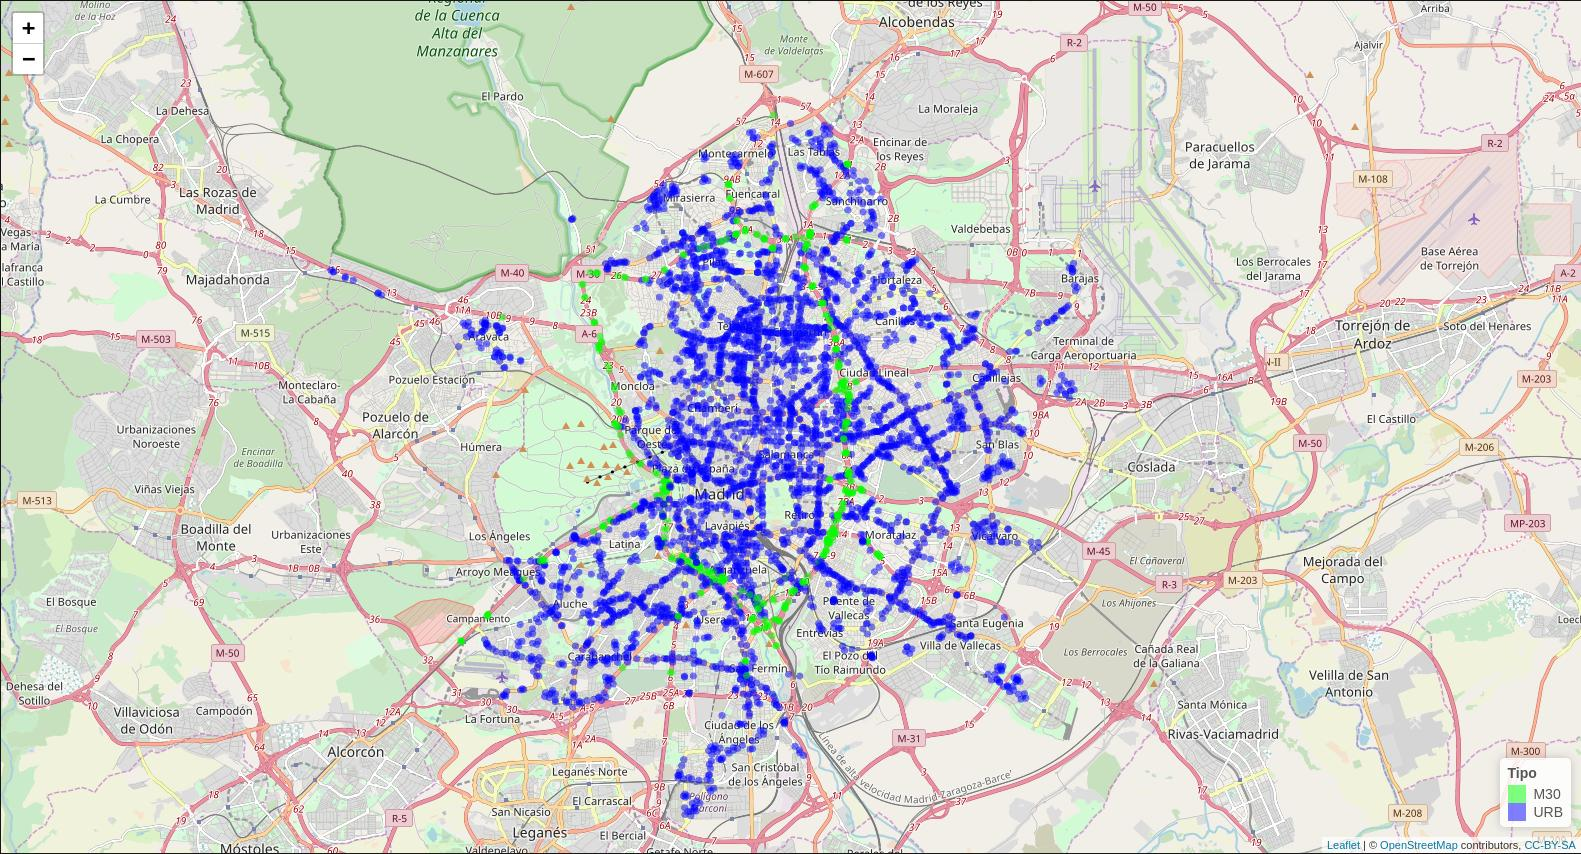
\includegraphics[width=1\linewidth]{images/locations_2018_09} \caption{Mapa de localización de los Puntos de Medida (Septiembre 2018)}\label{fig:locations-map}
\end{figure}

\subsection{Análisis de corrupción de los datos de
localización}\label{analisis-de-corrupcion-de-los-datos-de-localizacion}

Al igual que con los datos de medidas, podemos observar en qué meses se
han informado localizaciones de los dispositivos de medida (Cuadro
\ref{tab:locations-year-month-freq}).

\begin{longtable}{rrr}
\caption{\label{tab:locations-year-month-freq}Dispositivos que informan localización por año y mes}\\
\toprule
Año & Mes & Dispositivos\\
\midrule
\endfirsthead
\caption[]{\label{tab:locations-year-month-freq}Dispositivos que informan localización por año y mes \textit{(continued)}}\\
\toprule
Año & Mes & Dispositivos\\
\midrule
\endhead
\
\endfoot
\bottomrule
\endlastfoot
\rowcolor{gray!6}  2018 & 10 & 4119\\
2018 & 9 & 4117\\
\rowcolor{gray!6}  2018 & 8 & 4102\\
2018 & 7 & 4100\\
\rowcolor{gray!6}  2018 & 6 & 4103\\
\addlinespace
2018 & 4 & 4101\\
\rowcolor{gray!6}  2018 & 3 & 4078\\
2018 & 2 & 4078\\
\rowcolor{gray!6}  2018 & 1 & 4072\\
2017 & 12 & 4073\\
\addlinespace
\rowcolor{gray!6}  2017 & 11 & 4067\\
2017 & 10 & 4058\\*
\end{longtable}

En particular, resulta interesante estudiar cuánto ha variado el valor
de localización por dispositivo a lo largo del tiempo.

Hemos comprobado que \textbf{considerando todo el histórico de
localizaciones} de terminales, \textbf{4.065 de los 4.141} se han visto
\textbf{sometidos a cambios superiores a 1 unidad en sus coordenadas de
localización} (Cuadro \ref{tabs:all-locations-diff-summary}).

\begin{longtable}[]{@{}llllll@{}}
\caption{\label{tabs:all-locations-diff-summary}Resumen de dispositivos
cuya variación en la localización es superior a la unidad (todo el
histórico de datos)}\tabularnewline
\toprule
\begin{minipage}[b]{0.05\columnwidth}\raggedright\strut
No\strut
\end{minipage} & \begin{minipage}[b]{0.11\columnwidth}\raggedright\strut
Variable\strut
\end{minipage} & \begin{minipage}[b]{0.28\columnwidth}\raggedright\strut
Estadístico / Valor\strut
\end{minipage} & \begin{minipage}[b]{0.21\columnwidth}\raggedright\strut
Freqs (\% Válidos)\strut
\end{minipage} & \begin{minipage}[b]{0.08\columnwidth}\raggedright\strut
Válidos\strut
\end{minipage} & \begin{minipage}[b]{0.08\columnwidth}\raggedright\strut
Perdidos\strut
\end{minipage}\tabularnewline
\midrule
\endfirsthead
\toprule
\begin{minipage}[b]{0.05\columnwidth}\raggedright\strut
No\strut
\end{minipage} & \begin{minipage}[b]{0.11\columnwidth}\raggedright\strut
Variable\strut
\end{minipage} & \begin{minipage}[b]{0.28\columnwidth}\raggedright\strut
Estadístico / Valor\strut
\end{minipage} & \begin{minipage}[b]{0.21\columnwidth}\raggedright\strut
Freqs (\% Válidos)\strut
\end{minipage} & \begin{minipage}[b]{0.08\columnwidth}\raggedright\strut
Válidos\strut
\end{minipage} & \begin{minipage}[b]{0.08\columnwidth}\raggedright\strut
Perdidos\strut
\end{minipage}\tabularnewline
\midrule
\endhead
\begin{minipage}[t]{0.05\columnwidth}\raggedright\strut
1\strut
\end{minipage} & \begin{minipage}[t]{0.11\columnwidth}\raggedright\strut
id\\
{[}entero{]}\strut
\end{minipage} & \begin{minipage}[t]{0.28\columnwidth}\raggedright\strut
Media (sd) : 5701.7 (1852.8)\\
min \textless{} med \textless{} max:\\
0 \textless{} 5450 \textless{} 10337\\
IQR (CV) : 2083 (0.3)\strut
\end{minipage} & \begin{minipage}[t]{0.21\columnwidth}\raggedright\strut
4065 diferentes\strut
\end{minipage} & \begin{minipage}[t]{0.08\columnwidth}\raggedright\strut
4065\\
(100\%)\strut
\end{minipage} & \begin{minipage}[t]{0.08\columnwidth}\raggedright\strut
0\\
(0\%)\strut
\end{minipage}\tabularnewline
\begin{minipage}[t]{0.05\columnwidth}\raggedright\strut
2\strut
\end{minipage} & \begin{minipage}[t]{0.11\columnwidth}\raggedright\strut
x\_diff\\
{[}numerico{]}\strut
\end{minipage} & \begin{minipage}[t]{0.28\columnwidth}\raggedright\strut
Media (sd) : 109.3 (4.4)\\
min \textless{} med \textless{} max:\\
0.5 \textless{} 109.4 \textless{} 146.1\\
IQR (CV) : 0 (0)\strut
\end{minipage} & \begin{minipage}[t]{0.21\columnwidth}\raggedright\strut
4065 diferentes\strut
\end{minipage} & \begin{minipage}[t]{0.08\columnwidth}\raggedright\strut
4065\\
(100\%)\strut
\end{minipage} & \begin{minipage}[t]{0.08\columnwidth}\raggedright\strut
0\\
(0\%)\strut
\end{minipage}\tabularnewline
\begin{minipage}[t]{0.05\columnwidth}\raggedright\strut
3\strut
\end{minipage} & \begin{minipage}[t]{0.11\columnwidth}\raggedright\strut
y\_diff\\
{[}numerico{]}\strut
\end{minipage} & \begin{minipage}[t]{0.28\columnwidth}\raggedright\strut
Meadia (sd) : 207.4 (9.5)\\
min \textless{} med \textless{} max:\\
1.2 \textless{} 207.5 \textless{} 426.1\\
IQR (CV) : 0 (0)\strut
\end{minipage} & \begin{minipage}[t]{0.21\columnwidth}\raggedright\strut
4064 diferentes 4 (\strut
\end{minipage} & \begin{minipage}[t]{0.08\columnwidth}\raggedright\strut
065\\
100\%)\strut
\end{minipage} & \begin{minipage}[t]{0.08\columnwidth}\raggedright\strut
0\\
(0\%)\strut
\end{minipage}\tabularnewline
\bottomrule
\end{longtable}

Sin embargo, considerando sólo \textbf{datos de localización de los
terminales desde Noviembre de 2017}, vemos que \textbf{sólo 18
dispositivos} tienen cambios significativos en sus coordenadas de
localización (Cuadro
\ref{tabs:all-locations-diff-from-november-summary}).

\begin{longtable}[]{@{}llllll@{}}
\caption{\label{tabs:all-locations-diff-from-november-summary}Resumen de
dispositivos cuya variación en la localización es superior a la unidad
(desde Noviembre de 2017)}\tabularnewline
\toprule
\begin{minipage}[b]{0.05\columnwidth}\raggedright\strut
No\strut
\end{minipage} & \begin{minipage}[b]{0.11\columnwidth}\raggedright\strut
Variable\strut
\end{minipage} & \begin{minipage}[b]{0.29\columnwidth}\raggedright\strut
Estadístico / Valor\strut
\end{minipage} & \begin{minipage}[b]{0.20\columnwidth}\raggedright\strut
Freqs (\% Válidos)\strut
\end{minipage} & \begin{minipage}[b]{0.08\columnwidth}\raggedright\strut
Válidos\strut
\end{minipage} & \begin{minipage}[b]{0.08\columnwidth}\raggedright\strut
Perdidos\strut
\end{minipage}\tabularnewline
\midrule
\endfirsthead
\toprule
\begin{minipage}[b]{0.05\columnwidth}\raggedright\strut
No\strut
\end{minipage} & \begin{minipage}[b]{0.11\columnwidth}\raggedright\strut
Variable\strut
\end{minipage} & \begin{minipage}[b]{0.29\columnwidth}\raggedright\strut
Estadístico / Valor\strut
\end{minipage} & \begin{minipage}[b]{0.20\columnwidth}\raggedright\strut
Freqs (\% Válidos)\strut
\end{minipage} & \begin{minipage}[b]{0.08\columnwidth}\raggedright\strut
Válidos\strut
\end{minipage} & \begin{minipage}[b]{0.08\columnwidth}\raggedright\strut
Perdidos\strut
\end{minipage}\tabularnewline
\midrule
\endhead
\begin{minipage}[t]{0.05\columnwidth}\raggedright\strut
1\strut
\end{minipage} & \begin{minipage}[t]{0.11\columnwidth}\raggedright\strut
id\\
{[}entero{]}\strut
\end{minipage} & \begin{minipage}[t]{0.29\columnwidth}\raggedright\strut
Media (sd) : 6726.6 (2118.2)\\
min \textless{} med \textless{} max:\\
3714 \textless{} 6229 \textless{} 10280\\
IQR (CV) : 1782 (0.3)\strut
\end{minipage} & \begin{minipage}[t]{0.20\columnwidth}\raggedright\strut
18 diferentes\strut
\end{minipage} & \begin{minipage}[t]{0.08\columnwidth}\raggedright\strut
18\\
(100\%)\strut
\end{minipage} & \begin{minipage}[t]{0.08\columnwidth}\raggedright\strut
0\\
(0\%)\strut
\end{minipage}\tabularnewline
\begin{minipage}[t]{0.05\columnwidth}\raggedright\strut
2\strut
\end{minipage} & \begin{minipage}[t]{0.11\columnwidth}\raggedright\strut
x\_diff\\
{[}numerico{]}\strut
\end{minipage} & \begin{minipage}[t]{0.29\columnwidth}\raggedright\strut
Media (sd) : 8.4 (8.8)\\
min \textless{} med \textless{} max:\\
0.2 \textless{} 4.8 \textless{} 35.1\\
IQR (CV) : 8.9 (1)\strut
\end{minipage} & \begin{minipage}[t]{0.20\columnwidth}\raggedright\strut
18 diferentes\strut
\end{minipage} & \begin{minipage}[t]{0.08\columnwidth}\raggedright\strut
18\\
(100\%)\strut
\end{minipage} & \begin{minipage}[t]{0.08\columnwidth}\raggedright\strut
0\\
(0\%)\strut
\end{minipage}\tabularnewline
\begin{minipage}[t]{0.05\columnwidth}\raggedright\strut
3\strut
\end{minipage} & \begin{minipage}[t]{0.11\columnwidth}\raggedright\strut
y\_diff\\
{[}numerico{]}\strut
\end{minipage} & \begin{minipage}[t]{0.29\columnwidth}\raggedright\strut
Media (sd) : 5.3 (4.1)\\
min \textless{} med \textless{} max:\\
0.9 \textless{} 4.5 \textless{} 13.4\\
IQR (CV) : 7.1 (0.8)\strut
\end{minipage} & \begin{minipage}[t]{0.20\columnwidth}\raggedright\strut
18 diferentes\strut
\end{minipage} & \begin{minipage}[t]{0.08\columnwidth}\raggedright\strut
18\\
(100\%)\strut
\end{minipage} & \begin{minipage}[t]{0.08\columnwidth}\raggedright\strut
0\\
(0\%)\strut
\end{minipage}\tabularnewline
\bottomrule
\end{longtable}

\textbf{Esto claramente nos indica que los datos de localización
históricos están corruptos.}

Conclusiones:

\begin{itemize}
\tightlist
\item
  \textbf{los datos históricos de localización sólo son válidos a partir
  de Noviembre de 2017}
\item
  \textbf{desde Noviembre de 2017, sólo son fiables los datos de
  localización del 98,5\% de los terminales}
\item
  \textbf{los terminales que caen en el 1,5\% cuya localización padece
  de modificaciones desde Noviembre de 2017 los vamos a descartar} en
  nuestro estudio, por alguna de las siguientes razones:

  \begin{itemize}
  \tightlist
  \item
    porque su localización esté corrupta en el histórico de
    localizaciones
  \item
    porque verdaderamente hayan podido cambiar de localización a lo
    largo del tiempo, lo cual implicaría una complejidad excesiva en el
    resto de esta investigación
  \end{itemize}
\end{itemize}

\section{Selección de la propiedad objeto de
estudio}\label{seleccion-de-la-propiedad-objeto-de-estudio}

El objetivo principal de este trabajo es pronosticar el flujo de tráfico
en la ciudad de Madrid.

De las propiedades que ofrece el conjunto de datos de medidas tomadas
por los dispositivos de medida, las siguientes podrían servir para
describir el estado en el que se encuentra el tráfico en un punto dado:

\begin{itemize}
\tightlist
\item
  \textbf{intensidad}: intensidad del punto de medida en el periodo de
  15 minutos (vehículos/hora).
\item
  \textbf{ocupacion}: tiempo de ocupación del punto de medida en el
  periodo de 15 minutos (\%).
\item
  \textbf{carga}: carga de vehículos en el periodo de 15 minutos.
  Parámetro que tiene en cuenta intensidad, ocupación y capacidad de la
  vía y establece el grado de uso de la vía de 0 a 100.
\item
  \textbf{vmed}: velocidad media de los vehículos en el periodo de 15
  minutos (Km./h). Sólo para puntos de medida interurbanos M30.
\end{itemize}

En primer lugar, \textbf{descartamos} como propiedad objetivo la
velocidad media \textbf{vmed}, puesto que este valor solamente se
informa para los dispositivos de la \textbf{M30} y en este estudio se
pretende un modelo que pronostique el flujo en cualquier punto de la
ciudad (también los urbanos).

De las 3 restantes, realmente sería la \textbf{carga} la propiedad más
importante a pronosticar, por tres razones:

\begin{itemize}
\tightlist
\item
  se corresponde con un valor que tiene \textbf{significado directo
  sobre la ocupación del punto}
\item
  \textbf{se expresa como un porcentaje}, de manera que intuitivamente
  es \textbf{fácil de entender} (independiente del contexto o
  peculiaridades del lugar en el que esté el punto de medida)
\item
  es un valor ya cocinado, por lo que una vez pronosticado, no requiere
  de mayor transformación
\end{itemize}

Para disponer de información suficiente que permita validar que la
propiedad \textbf{carga} es la mejor candidata, se ha revisado que la
cantidad relativa de veces que no ha sido informada no sea excesivamente
superior a cualquier otra propiedad. En caso contrario, es decir,
\textbf{caso que los datos informados en la propiedad carga realmente
fuesen muy precarios, tal vez sería conveniente no seleccionar esta como
la propiedad objetivo} e intentar adoptar otros enfoques.

Este estudio se ha realizado con los datos de 2018 recogidos por todos
los puntos de medida. Para esta labor se ha utilizado el paquete
\emph{imputeTS} \citep{imputeTS2018} de R. El resultado, con la cantidad
relativa de veces que cada propiedad no ha sido informada de forma
correcta se muestra en el Cuadro \ref{tabs:nas-2018}.

\begin{longtable}[]{@{}llllll@{}}
\caption{\label{tabs:nas-2018}Resumen de valores reportados erróneamente
en 2018 para las propiedades intensidad, ocupación y
carga}\tabularnewline
\toprule
\begin{minipage}[b]{0.04\columnwidth}\raggedright\strut
No\strut
\end{minipage} & \begin{minipage}[b]{0.18\columnwidth}\raggedright\strut
Variable\strut
\end{minipage} & \begin{minipage}[b]{0.24\columnwidth}\raggedright\strut
Estadístico / Valor\strut
\end{minipage} & \begin{minipage}[b]{0.20\columnwidth}\raggedright\strut
Freqs (\% Válidos)\strut
\end{minipage} & \begin{minipage}[b]{0.08\columnwidth}\raggedright\strut
Válidos\strut
\end{minipage} & \begin{minipage}[b]{0.08\columnwidth}\raggedright\strut
Perdidos\strut
\end{minipage}\tabularnewline
\midrule
\endfirsthead
\toprule
\begin{minipage}[b]{0.04\columnwidth}\raggedright\strut
No\strut
\end{minipage} & \begin{minipage}[b]{0.18\columnwidth}\raggedright\strut
Variable\strut
\end{minipage} & \begin{minipage}[b]{0.24\columnwidth}\raggedright\strut
Estadístico / Valor\strut
\end{minipage} & \begin{minipage}[b]{0.20\columnwidth}\raggedright\strut
Freqs (\% Válidos)\strut
\end{minipage} & \begin{minipage}[b]{0.08\columnwidth}\raggedright\strut
Válidos\strut
\end{minipage} & \begin{minipage}[b]{0.08\columnwidth}\raggedright\strut
Perdidos\strut
\end{minipage}\tabularnewline
\midrule
\endhead
\begin{minipage}[t]{0.04\columnwidth}\raggedright\strut
1\strut
\end{minipage} & \begin{minipage}[t]{0.18\columnwidth}\raggedright\strut
\% intensidad NAs\\
{[}numerico{]}\strut
\end{minipage} & \begin{minipage}[t]{0.24\columnwidth}\raggedright\strut
media (sd) : 0.04 (0.09)\\
min \textless{} med \textless{} max :\\
0 \textless{} 0.02 \textless{} 1\\
IQR (CV) : 0.03 (2.13)\strut
\end{minipage} & \begin{minipage}[t]{0.20\columnwidth}\raggedright\strut
934 diferentes\strut
\end{minipage} & \begin{minipage}[t]{0.08\columnwidth}\raggedright\strut
2906\\
(100\%)\strut
\end{minipage} & \begin{minipage}[t]{0.08\columnwidth}\raggedright\strut
0\\
(0\%)\strut
\end{minipage}\tabularnewline
\begin{minipage}[t]{0.04\columnwidth}\raggedright\strut
2\strut
\end{minipage} & \begin{minipage}[t]{0.18\columnwidth}\raggedright\strut
\% ocupacion NAs\\
{[}numerico{]}\strut
\end{minipage} & \begin{minipage}[t]{0.24\columnwidth}\raggedright\strut
media (sd) : 0.08 (0.1)\\
min \textless{} med \textless{} max :\\
0 \textless{} 0.05 \textless{} 1\\
IQR (CV) : 0.05 (1.25)\strut
\end{minipage} & \begin{minipage}[t]{0.20\columnwidth}\raggedright\strut
1315 diferentes\strut
\end{minipage} & \begin{minipage}[t]{0.08\columnwidth}\raggedright\strut
2906\\
(100\%)\strut
\end{minipage} & \begin{minipage}[t]{0.08\columnwidth}\raggedright\strut
0\\
(0\%)\strut
\end{minipage}\tabularnewline
\begin{minipage}[t]{0.04\columnwidth}\raggedright\strut
3\strut
\end{minipage} & \begin{minipage}[t]{0.18\columnwidth}\raggedright\strut
\% carga NAs\\
{[}numerico{]}\strut
\end{minipage} & \begin{minipage}[t]{0.24\columnwidth}\raggedright\strut
media (sd) : 0.05 (0.1)\\
min \textless{} med \textless{} max :\\
0 \textless{} 0.02 \textless{} 1\\
IQR (CV) : 0.04 (1.86)\strut
\end{minipage} & \begin{minipage}[t]{0.20\columnwidth}\raggedright\strut
986 diferentes\strut
\end{minipage} & \begin{minipage}[t]{0.08\columnwidth}\raggedright\strut
2906\\
(100\%)\strut
\end{minipage} & \begin{minipage}[t]{0.08\columnwidth}\raggedright\strut
0\\
(0\%)\strut
\end{minipage}\tabularnewline
\bottomrule
\end{longtable}

Vemos que el porcentaje en el que la propiedad \textbf{carga} no está
informada correctamente es menor que el homólogo para
\textbf{ocupación}. Y no es mucho mayor que el correspondiente valor de
la propiedad \textbf{intensidad}.

Por lo tanto, los datos no contravienen el objetivo de pronosticar la
propiedad carga, que es la más relevante para este estudio por las
razones expuestas más arriba.

Podemos ver la distribución de los porcentajes de datos faltantes en las
series de carga reportadas por los dispositivos en todo el histórico de
datos en la Figura \ref{fig:all-gaps-hist}.

\emph{Nótese que es diferente el análisis de calidad realizado en los
párrafos anteriores (medidas recibidas sin valor de carga, intensidad u
ocupación), que el análisis al que se refiere la Figura
\ref{fig:all-gaps-hist} (``huecos'' en la serie temporal en la que no se
han recibido datos, ni de carga ni de ninguna otra propiedad).}

\begin{figure}

{\centering \includegraphics[width=0.6\linewidth]{307.datos.propiedad.objetivo_files/figure-latex/all-gaps-hist-1} 

}

\caption{Histograma del porcentaje de datos faltantes en los datos reportados por todos los dispositivos}\label{fig:all-gaps-hist}
\end{figure}

\section{Análisis exploratorio de la propiedad
carga}\label{analisis-exploratorio-de-la-propiedad-carga}

Es importante determinar de forma heurística el patrón estacional que
puedan presentar los datos que vamos a estudiar. De especial ayuda son
los gráficos de representación polar para esta tarea.

Con esta finalidad se han explorado las series de carga reportadas por
varios dispositivos. En la Figura \ref{fig:4000-multi-seasonal} pueden
verse las distintas estacionalidades que presenta la propiedad carga
para uno de estos dispositivos, sirviendo de generalidad para lo
observado en el resto de ellos.

\begin{figure}

{\centering \includegraphics[width=1\linewidth]{308.datos.descripcion.carga_files/figure-latex/4000-multi-seasonal-1} 

}

\caption{Gráfico de diferentes estacionalidades de la carga (dispositivo 4000)}\label{fig:4000-multi-seasonal}
\end{figure}

Podemos observar que las series tiene componentes estacionales diarias,
semanales y anuales; circunstancia por otro lado bastante natural dada
la relación directa entre el flujo de tráfico de una ciudad y el
calendario por el que se gobierna la actividad humana.

\section{Fallas en los datos}\label{fallas-en-los-datos}

La mayoría de los algoritmos de modelado y pronóstico de series
temporales requieren de datos que no tengan fallas.

Para tener una idea de lo significativas que pueden llegar a ser estas
anomalías en los datos tomados por los dispositivos, podemos observar
por ejemplo las medidas tomadas por el dispositivo 10.329 en la primera
semana de Julio de 2.018 en la Figura \ref{fig:gaps-10329}.

\begin{figure}

{\centering \includegraphics[width=0.6\linewidth]{308.datos.descripcion.carga_files/figure-latex/gaps-10329-1} 

}

\caption{Fallas en los datos informados por el dispositivo 10.329 en Julio de 2018}\label{fig:gaps-10329}
\end{figure}

Dependiendo del tipo de algoritmo utilizado en cada caso, se ha
seleccionado la técnica más conveniente para la reparación de estas
fallas. Por ahora, para el estudio exploratorio de la propiedad
\emph{carga} (principalmente en lo relativo a su estacionalidad) hemos
utilizado técnicas muy sencillas, como acarrear el último valor conocido
o \textbf{interpolar con los valores extremos}.

Es importante tener en cuenta, que para fallas grandes no será fácil
reparar los datos de una manera no nociva. Tarea ésta que por otro lado
supone un área de investigación y que excede los límites de este
trabajo.

\chapter{Métodos paramétricos}\label{metodos-parametricos}

\section{Fundamentos}\label{fundamentos}

Una \textbf{serie temporal} es una secuencia de datos, observaciones o
valores, medidos en determinados momentos y ordenados cronológicamente.
Los datos pueden estar espaciados a intervalos iguales (como la
temperatura en un observatorio meteorológico en días sucesivos a una
determinada hora) o desiguales (como el peso de una persona en sucesivas
mediciones a lo largo de su vida).

Para el análisis de series temporales se usan métodos que ayudan a
interpretarlas y que permiten extraer información representativa sobre
las relaciones subyacentes entre los datos de la serie. Estos métodos
pueden extrapolar o interpolar los datos y así predecir el
comportamiento de la serie en momentos no observados, ya sea en el
futuro (extrapolación para pronóstico), en el pasado (extrapolación
retrógrada) o en momentos intermedios (interpolación).

El \textbf{análisis clásico} de las series temporales se basa en que los
valores que toma la variable de observación es la consecuencia de cuatro
componentes, cuya actuación conjunta da como resultado los valores
medidos.

Estas componentes son:

\begin{itemize}
\item
  \textbf{Tendencia}. Es la marcha general y persistente del fenómeno
  observado. Es una componente de la serie que refleja la evolución a
  largo plazo. Cuando se hace referencia a la ``tendencia'' en los datos
  de series de tiempo, significa que los datos tienen una trayectoria a
  largo plazo que puede ser una tendencia en la dirección positiva o
  negativa. Un ejemplo de tendencia sería un aumento a largo plazo de
  los datos de ventas de una empresa.
\item
  \textbf{Estacionalidad}. Es el movimiento periódico de corto plazo. Se
  trata de una componente causal debida a la influencia de ciertos
  fenómenos que se repiten de manera periódica en un año (las
  estaciones), una semana (los fines de semana), un día (las horas
  punta) o cualquier otro periodo. Recoge las oscilaciones que se
  producen en esos períodos de repetición.
\item
  \textbf{Ciclo}. Es la componente de la serie que recoge las
  oscilaciones periódicas de amplitud superior a un año. Movimientos
  normalmente irregulares alrededor de la tendencia, en las que a
  diferencia de las variaciones estacionales, tiene un período y
  amplitud variables, pudiendo clasificarse como cíclicos, cuasi
  cíclicos o recurrentes. Son períodos de repetición que no están
  relacionados con el calendario. Un ejemplo de esta componente son los
  ciclos económicos, como recesiones o expansiones económicas, pero que
  no están relacionados con el calendario en el sentido semanal, mensual
  o anual.
\item
  \textbf{Variación aleatoria o ruido}, accidental, de carácter
  errático, también denominada \textbf{residuo}, no muestra ninguna
  regularidad (salvo las regularidades estadísticas). Es la componente
  irregular e \textbf{impredecible} de la serie, que describe las
  influencias aleatorias de la misma. Representa los residuos, es decir,
  lo que queda de la serie temporal después de que se hayan eliminado
  las otras componentes.
\end{itemize}

Algunos autores hablan además de otra componente:

\begin{itemize}
\tightlist
\item
  \textbf{Variación accidental}, de carácter errático debida a fenómenos
  aislados que son capaces de modificar el comportamiento de la serie
  (tendencia, estacionalidad, variaciones cíclicas y aleatoria).
\end{itemize}

Suele ser habitual que los algoritmos de pronóstico de series temporales
fusionen las componentes de tendencia y ciclo en una sóla, de manera que
las descomposiciones resultantes acaban estando compuestas de
tendencia-ciclo, estacionalidad y ruido.

En el lenguaje de programación \emph{R} las series temporales suelen
trabajarse con el objeto \emph{ts}. La \textbf{frecuencia} es el número
de observaciones que se registran en un mismo patrón estacional. De este
modo, cuando se define una serie temporal no sólo se indica la secuencia
de números que la componen sino también la frecuencia que presenta esa
secuencia.

Según el enfoque clásico, hay tres tipos de series temporales:

\begin{itemize}
\item
  \textbf{Series aditivas}, que se componen sumando tendencia,
  estacionalidad y ruido.

  \(X_{t} = T_{t} + E_{t} + R_{t}\)
\item
  \textbf{Series multiplicativas}, que se componen multiplicando
  tendencia, estacionalidad y ruido:

  \(X_{t} = T_{t} \cdot E_{t} \cdot R_{t}\)
\item
  \textbf{Series mixtas}, que se componen sumando y multiplicando (hay
  distintas variantes) tendencia, estacionalidad y ruido.
\end{itemize}

La \textbf{notación} más habitual para trabajar con series temporales
suele ser:

\[X = \{X_{1},X_{2},\dots \} \text{ o } \{X_{k}\}_{k\geq 1}\]

También es frecuente expresarlas del modo:

\[Y = \{Y_{t}:t\in T\ \}\]

La \textbf{descomposición} es la de-construcción de los datos crudos de
la serie en sus diversos componentes: tendencia, estacionalidad-ciclo y
ruido (si existieran). Dependiendo de la serie, la descomposición será
multiplicativa o aditiva.

El propósito de la descomposición es aislar los distintos componentes
para que se puedan ver individualmente y realizar el análisis o
pronósticos sin la influencia del ruido o la estacionalidad. Por
ejemplo, si solo se desea ver la tendencia de una serie, hay que
eliminar la estacionalidad que se encuentra en los datos, el ruido
debido a la aleatoriedad y cualquier ciclo como la expansión económica.

Un ejemplo aplicado a nuestros datos tomados por los dispositivos de
medida lo podemos ver en la Figura \ref{fig:stl-diario}. En esta figura
se define la serie con frecuencia diaria (4*24 registros por estación).
Vemos que la tendencia tiene una variación que hace que se asemeje más
bien a una estacionalidad semanal. Es decir, modelando la serie
atendiendo únicamente a su componente estacional diaria vemos que el
resultado no es satisfactorio. Dicho de otro modo, el ciclo repetitivo
basado únicamente en la ventana de tiempo diaria no puede modelar los
patrones cíclicos semanales, que vemos que acaban influyendo la
componente de la tendencia.

\begin{figure}

{\centering \includegraphics[width=0.8\linewidth]{410.metodo.parametricos.fundamentos_files/figure-latex/stl-diario-1} 

}

\caption{Descomposición aditiva con estacionalidad diaria para los datos reportados por el dispositivo 4.000 en el verano de 2018.}\label{fig:stl-diario}
\end{figure}

Veamos en la Figura \ref{fig:stl-semanal} la descomposición considerando
una frecuencia semanal (4*24*7 registros por estación). En este caso
vemos que efectivamente la componente de estacionalidad realmente parece
un patrón que se repite de forma estacional y vemos también como la
tendencia es una línea que describe la evolución a más largo plazo que
la estación.

\begin{figure}

{\centering \includegraphics[width=0.8\linewidth]{410.metodo.parametricos.fundamentos_files/figure-latex/stl-semanal-1} 

}

\caption{Descomposición aditiva con estacionalidad semanal para los datos reportados por el dispositivo 4.000 en el verano de 2018.}\label{fig:stl-semanal}
\end{figure}

Por lo tanto, tal como ya vimos en el análisis de estacionalidad de la
carga, es conveniente tener en consideración también las
estacionalidades semanal y anual.

\section{Método STL con estacionalidad
única}\label{metodo-stl-con-estacionalidad-unica}

\textbf{STL} es un método versátil y robusto para descomponer series
temporales. STL es un acrónimo de ``Descomposición estacional y de
tendencias con Loess'', siendo Loess un método para estimar relaciones
no lineales. El método STL fue desarrollado por Cleveland, McRae y
Terpenning \citep{cleveland1990stl} .

En el lenguaje \emph{R} podemos realizar una descomposición \emph{stl}
utilizando el paquete \emph{stats}. Es importante notar que \textbf{este
método no permite series con estacionalidad múltiple}. Más adelante
veremos otros métodos que sí permiten series que presentan varios
patrones de estacionalidad.

Los dos parámetros principales que se deben elegir cuando se usa
\textbf{STL} son la ventana del ciclo-tendencia (t.window) y la ventana
estacional (s.window). Estos parámetros controlan la rapidez con la que
pueden cambiar las componentes de tendencia y estacionalidad. Valores
pequeños permiten cambios más rápidos y valores grandes producen modelos
con cambios más moderados en estas componentes. Ambos t.window y
s.window deben ser números impares;

\begin{itemize}
\tightlist
\item
  t.window es el número de observaciones consecutivas que se utilizarán
  al estimar la tendencia-ciclo.
\item
  s.window es el número de períodos consecutivos que se utilizarán para
  estimar cada valor en la componente estacional.
\end{itemize}

Si bien la descomposición es principalmente útil para estudiar datos de
las series y para explorar cambios históricos a lo largo del tiempo,
también se puede utilizar para pronosticar.

Para utilizar la descomposición STL para hacer pronósticos se procede
del siguiente modo:

\begin{itemize}
\tightlist
\item
  la componente estacional se pronostica tomando la observación
  correspondiente del periodo inmediatamente anterior
\item
  la componente compuesta por tendencia y ruido se suele pronosticar por
  cualquier algoritmo no estacional
\end{itemize}

Afortunadamente, el paquete \emph{forecast} de \emph{R} realiza todo
este trabajo de forma transparente.

Hemos desarrollado una buena batería de funciones que permiten
contrastar de forma rápida los pronósticos según distintos algoritmos y
representar visualmente los resultados. Utilizando estas funciones y
considerando los datos reportados en 2018 por el dispositivo 4.000,
podemos poner a prueba la capacidad de pronóstico del algoritmo STL.

En la Figura \ref{fig:stl-4000-ex-1} observamos pronósticos realizados
considerando la serie con estacionalidad \emph{diaria, semanal, mensual}
y \emph{anual}. Hemos hecho pruebas considerando todos los datos
reportados por el dispositivo (133.302 valores) y también considerando
únicamente los últimos datos recientes valores de la serie (20.000
valores).

Nótese como los pronósticos basados en estacionalidad diaria son
bastante menos acertados para días de fin de semana; se entiende que el
modelo tiende a acomodarse al comportamiento mayoritario día a día (5
días laborables a la semana son más del doble que 2 días no laborables).
Esta tara vemos como queda bastante mejor corregida en el caso del
modelo ajustado teniendo en cuenta estacionalidad semanal.

\begin{figure}[htbp]
\centering
\includegraphics{411.metodo.parametricos.stl_files/figure-latex/stl-4000-ex-1-1.pdf}
\caption{\label{fig:stl-4000-ex-1}Ejemplo de pronósticos a 48 horas vista
con el algoritmo STL para la serie reportada por el dispositivo 4.000
utilizando estacionalidad diaria, semanal, mensual o anual, considerando
toda la serie o sólamente los 20.000 valores más recientes de la misma}
\end{figure}

Visualmente vemos que los resultados son mejorables aunque es difícil
determinar qué tipo de estacionalidad, diaria o semanal, ofrece mejor
rendimiento de pronóstico. \textbf{Las estacionalidades mensual y anual
claramente se delatan como no apropiadas} (seguramente por no coincidir
el patrón mensual o anual con el semanal, que es el más influyente en el
caso del flujo de tráfico).

Más tarde, en el apartado de resultados, veremos la capacidad de
pronóstico de este algoritmo comparada con el resto de métodos que
ponemos a prueba en este trabajo.

\section{Método MSTL - STL
multiestacional}\label{metodo-mstl---stl-multiestacional}

En series como las del flujo de tráfico es natural observar que las
estacionalidades son varias:

\begin{itemize}
\tightlist
\item
  \textbf{diaria}, pues no a todas horas el flujo es igual.
\item
  \textbf{semanal}, ya que según el día de la semana es normal que el
  tráfico fluya más o menos y en distintas regiones.
\item
  \textbf{anual}, puesto que los periodos vacacionales, por ejemplo,
  claramente condicionan los flujos de tráfico.
\end{itemize}

Puede también considerarse una estacionalidad mensual, pero en el caso
de los algoritmos STL y de nuestras series, no parece que ayude mucho,
como hemos comentado en el punto anterior.

El paquete \emph{forecast} de \emph{R} ofrece una extensión del
algoritmo STL con la que se puede aplicar pronósticos a series que
presentan estacionalidad múltiple, cómo es el caso de nuestras series de
estudio.

El algoritmo \textbf{MSTL} nuevamente descompone la serie en tendencia,
estacionalidad y ruido. Sin embargo, en este caso en lugar de modelar
una única estacionalidad, construye un modelo basado en tantas como
indiquemos que tiene nuestra serie (series multi-estacionales). Las
componentes estacionales se estiman de forma iterativa utilizando
\emph{STL}. La componente de tendencia se calcula en la última iteración
de STL. En el caso de que las series fueran no estacionales, este método
las descompone en tendencia y resto solamente. A diferencia de stl, en
el paquete \emph{forecast} mstl está completamente automatizado, lo cual
significa que la estimación de los metaparámetros óptimos la realiza el
propio algoritmo.

Podemos ver un ejemplo de descomposición multiestacional en la Figura
\ref{fig:stlm-ex}.

\begin{figure}

{\centering \includegraphics[width=0.8\linewidth]{412.metodo.parametricos.stlm_files/figure-latex/stlm-ex-1} 

}

\caption{Ejemplo de descomposición multiestacional: dispositivo 4.000, últimos 5.000 valores reportados, estacionalidades diaria y semanal}\label{fig:stlm-ex}
\end{figure}

Se han realizado el experimentos con estacionalidades \emph{diaria +
semanal}, \emph{diaria + semanal + mensual}, \emph{diaria + semanal +
anual} y \emph{diaria + semanal + mensual + anual} para todas las series
de dispositivos de medida. Puede verse el resultado de uno de los
experimentos para los datos reportados por el dispositivo 4.000 desde
2015 en la Figura \ref{fig:stlm-4000-ex}.

\begin{figure}

{\centering \includegraphics[width=1\linewidth]{412.metodo.parametricos.stlm_files/figure-latex/stlm-4000-ex-1} 

}

\caption{Ejemplo de pronósticos a 48 horas vista con el algoritmo MSTL para la serie reportada por el dispositivo 4.000 utilizando combinaciones de estacionalidad diaria, semanal, mensual o anual, considerando toda la serie o sólamente los 20.000 valores más recientes de la misma}\label{fig:stlm-4000-ex}
\end{figure}

Visualmente vemos que los resultados son muy prometedores. Pero no es
fácil determinar qué combinación de estacionalidades puede ser la más
productiva.

Más adelante, en el apartado de resultados de este capítulo, veremos
cómo se comporta este método comparado con STL aplicado a todas las
series que forman parte de este estudio.

\section{Método ARIMA}\label{metodo-arima}

Unos de los modelos clásicos más utilizados para el pronóstico de series
temporales son los \textbf{modelos ARIMA}. Los modelos ARIMA intentan
describir la auto correlación en los datos de la serie, por eso pueden
incluir términos \textbf{autorregresivos (AR)} y/o términos de
\textbf{media móvil MA} (traducido del término inglés ``moving
average''). Más adelante describiremos los modelos \textbf{SARIMA}
(ARIMA estacional), que también los utilizamos en nuestra investigación.

Pero antes de entrar en detalle en de los modelos ARIMA conviene hablar
de los conceptos de series estacionarias y diferenciación.

Una \textbf{serie temporal estacionaria} es aquella cuyas propiedades no
dependen del momento en que se observa la serie. Por lo tanto, las
series con tendencia, o con la estacionalidad, no son estacionarias: la
tendencia y la estacionalidad afectan al valor de la serie en diferentes
momentos.

Algunos casos pueden ser confusos: una serie temporal con comportamiento
cíclico (pero sin tendencia o estacionalidad) es estacionaria. Esto se
debe a que los ciclos no son de una longitud fija, por lo que antes de
observar las series no podemos estar seguros de dónde estarán los picos
y valles de los ciclos.

En general, una serie temporal estacionaria no tiene patrones
predecibles a largo plazo. Su representación gráfica mostrará que la
serie es aproximadamente horizontal (aunque es posible algún
comportamiento cíclico), con una variación constante.

Más concretamente, una serie \(\{y_t\}\) es estacionaria si la
distribución de \((y_t, ..., y_{t+s})\) no depende de \(t\) para todo
\(s\).

Típicamente, cuando una serie no es estacionaria, una forma de
transformarla en estacionaria es considerar los cambios de su valor en
el tiempo en lugar de observar los datos en crudo, esto es, calcular las
diferencias entre observaciones consecutivas. Esto se conoce como
\textbf{diferenciación}. \textbf{La diferenciación puede} ayudar a
estabilizar la media de una serie temporal y, por lo tanto,
\textbf{eliminar (o reducir) la tendencia y la estacionalidad}. Por otro
lado, para el caso de la varianza de la serie a lo largo del tiempo, a
veces suelen aplicarse transformaciones logarítmicas.

La serie diferenciada se corresponde con la variación entre
observaciones consecutivas en la serie original, y se puede escribir
como: \[y^{\prime}_t=y_t-y_{t-1}\]

En ocasiones, los datos diferenciados siguen siendo no estacionarios y
puede ser necesario diferenciar los datos una segunda vez para obtener
una serie estacionaria. En la práctica, casi nunca es necesario ir más
allá de las diferencias de segundo orden.

Una \textbf{diferencia estacional} es la diferencia entre una
observación y la observación anterior de la misma temporada. Es decir,
\[ y^{\prime}_t=y_t-y_{t-m}\] siendo \(m\) la longitud del periodo
estacional.

Es importante interpretar correctamente las diferencias. Las primeras
diferencias son el cambio entre una observación y la siguiente. Las
diferencias estacionales son el cambio entre un mismo momento de una
estación y el de la siguiente. Es poco probable que diferencias
realizadas sobre otros retrasos (no inmediatamente anterior ni
estacionales) tengan mucho sentido y deben evitarse.

Una forma de determinar de manera más objetiva si se requiere una
diferenciación es utilizar un \emph{test de raíz unitaria}. Son
contrastes de hipótesis estadísticas que juzgan la estacionariedad de
una serie para determinar si se requiere o no diferenciación. Por
ejemplo, la función \emph{adf.test} del paquete \emph{tseries} o la
función \emph{ur.kpss} del paquete \emph{urca} de R permiten realizar
este tipo de contrastes.

Hemos dicho que \textbf{los modelos ARIMA pueden tener una componente
basada en autorregresión}. En un modelo de autorregresión, se pronostica
la variable de interés utilizando una combinación lineal de valores
pasados de la variable. El término auto regresión indica que es una
regresión de la variable contra sí misma. Esta parte del modelo puede
expresarse con la fórmula:

\[y_{t} = c + \phi_{1}y_{t-1} + \phi_{2}y_{t-2} + \dots + \phi_{p}y_{t-p} + \varepsilon_{t}\]
dónde \(\varepsilon_{t}\) es ruido blanco, \(\phi_{i}\) son parámetros y
\(c\) es una constante. Este tipo de modelos suelen ser referidos como
\textbf{AR(p)}.

Normalmente los modelos autorregresivos requieren de series que sean
estacionarias. De ahí las aclaraciones sobre estacionariedad que hemos
realizado más arriba.

También hemos dicho más arriba que \textbf{los modelos ARIMA pueden
tener una componente basada en medias móviles}. Un modelo de media
móvil, en lugar de usar valores pasados de la variable de pronóstico en
una regresión, utiliza errores de pronóstico pasados en un modelo
similar a una regresión.

\[y_{t} = c + \varepsilon_t + \theta_{1}\varepsilon_{t-1} + \theta_{2}\varepsilon_{t-2} + \dots + \theta_{q}\varepsilon_{t-q},\]
dónde \(\varepsilon_{t}\) es ruido blanco, \(\theta_{i}\) son parámetros
y \(c\) es una constante. Este tipo de modelos suelen ser referidos como
\textbf{MA(q)}.

Si combinamos la diferenciación, la autorregresión y las medias móviles,
obtenemos un modelo ARIMA no estacional. ARIMA es un acrónimo de Media
Móvil Integrada Auto Regresiva (en este contexto, ``integración'' es lo
contrario de la diferenciación). El modelo completo se puede escribir
como:

\[ 
  y'_{t} = c + \phi_{1}y'_{t-1} + \cdots + \phi_{p}y'_{t-p} + \theta_{1}\varepsilon_{t-1} + \cdots + \theta_{q}\varepsilon_{t-q} + \varepsilon_{t}
\]

donde \(y'_{t}\) es la serie diferenciada (puede haber sido diferenciada
más de una vez), \(p\) es el orden de la parte autorregresiva, \(d\) es
el orden de la diferenciación y \(q\) es el orden de la parte de media
móvil.

La parte más complicada en la construcción de los modelos ARIMA es la
selección de los valores p, d, y q. A partir de una gráfica de la serie,
no suele ser posible determinar los valores correctos para estos
metaparámetros del modelo.

Sin embargo, para esta tarea suele ser muy útil valerse de las gráficas
ACF y PACF de la serie y sus diferencias.

\textbf{Las gráficas ACF} muestran las autocorrelaciones que miden la
relación entre \(y_t\) e \(y_{t-k}\) para diferentes valores de \(k\).
Sin embargo, estas gráficas no son suficientes porque si cada valor está
correlacionado con su predecesor, entonces también pueden existir
correlaciones entre un un valor cualquiera y el que precede a su
predecesor.

Para superar este problema, se utilizan las gráficas de autocorrelación
parcial. Éstas miden la relación entre \(y_t\) e \(y_{t-k}\) después de
eliminar los efectos de los retrasos \(1,2,...,k-1\).

Siguiendo las indicaciones de \citep{Forecast6-online}, tenemos la
heurística que se describe a continuación.

Los datos pueden seguir un modelo \textbf{ARIMA(p,d,0)} si los datos en
crudo presentan las siguientes características:

\begin{itemize}
\tightlist
\item
  la curva ACF cae de forma exponencial o sinusoidal
\item
  y hay un aumento significativo en el retraso p en la gráfica PACF,
  pero ninguno más allá del retraso p.
\end{itemize}

Los datos pueden seguir un modelo \textbf{ARIMA(0,d,q)} si los datos en
crudo satisfacen:

\begin{itemize}
\tightlist
\item
  la gráfica PACF cae de forma exponencial o sinusoidal
\item
  y hay un aumento significativo en el retraso q en el ACF, pero ninguno
  más allá del retraso q.
\end{itemize}

Por otro lado, según esta misma referencia, la heurística a seguir para
determinar los parámetros de un modelo ARIMA es:

\begin{enumerate}
\def\labelenumi{\arabic{enumi}.}
\tightlist
\item
  Representar los datos gráficamente.
\item
  Si es necesario, transformar los datos (utilizando una transformación
  de Box-Cox) para estabilizar la varianza.
\item
  Si los datos no son estacionarios, diferenciar hasta que los datos
  sean estacionarios.
\item
  Examinar las gráficas ACF/PACF: determinar si ARIMA(p,d,0) o
  ARIMA(0,d,q) son modelos apropiados según las indicaciones vistas más
  arriba.
\item
  Poner a prueba los modelos elegidos como prometedores.
\item
  Verificar los residuos del modelo elegido observando el ACF de los
  residuos. Si no se ven como ruido blanco, probar un modelo modificado.
\item
  Una vez que los residuos se vean como ruido blanco, el modelo es
  bueno.
\end{enumerate}

En la Figura \ref{fig:acf-pacf-4000} podemos ver las gráficas ACF y PACF
para nuestra serie de medidas tomadas por el dispositivo 4.000 a finales
de Septiembre de 2018.

\begin{figure}

{\centering \includegraphics[width=0.6\linewidth]{413.metodo.parametricos.arima_files/figure-latex/acf-pacf-4000-1} 

}

\caption{Original, ACF y PACF para los valores de carga del dispositivo 4.000 a finales de Septiembre de 2018}\label{fig:acf-pacf-4000}
\end{figure}

Según esta heurística, se han realizado distintas pruebas de ajuste de
modelos ARIMA no estacionales. En ningún caso se ha llegado a resultados
mínimamente satisfactorios.

Se ha utilizado incluso la función \emph{auto.arima} del paquete
\emph{forecast} de R, que realiza una búsqueda de modelos mucho más
exhaustiva sin haberse obtenido tampoco resultados que ofrezcan
rendimiento aceptable. En la Figura \ref{fig:arima-4000}, podemos ver un
ejemplo de pronóstico realizado con este método.

\begin{figure}

{\centering \includegraphics[width=0.6\linewidth]{413.metodo.parametricos.arima_files/figure-latex/arima-4000-1} 

}

\caption{Pronóstico del flujo de carga para el terminal 4.000 con ARIMA}\label{fig:arima-4000}
\end{figure}

Los resultados arrojados por este método, como decíamos, han sido
precarios. Sin embargo, no parece que sea una anomalía particular de
este estudio sino que son numerosos las referencias en las que este
comportamiento está documentado. Véase \citep{arima-sarima-lstm-online},
\citep{Forecast6-online}, etc. En general, parece que ARIMA (no
estacional) tiene buena capacidad de pronóstico a muy corto plazo, pero
en la medida en que incrementamos el horizonte de predicción su
rendimiento se ve perjudicado. Efectivamente, esto mismo ha ocurrido en
el caso de nuestros experimentos; para horizontes de entorno a los 15
minutos, las tasas de error son iguales o poco mayores que los mejores
de los métodos de este estudio, pero en la medida en que el horizonte
crece los resultados empeoran.

Nótese que en parte esto puede explicarse porque ARIMA (no estacional)
calcula los valores futuros a partir de los pasados, pero sólo de los
pasados recientes (no mucho más de los últimas 5 medidas reportadas,
parámetros p y q). Además, para calcular los instantes futuros, más allá
del primer instante, utiliza los valores pronosticados por el propio
modelo; es decir, en nuestro caso, para pronosticar el instante futuro
192 lo que hace es pronosticar el instante futuro de manera recursiva
192 veces, retroalimentándose en cada iteración con los instantes ya
calculados. Todo esto, de manera más intuitiva en este punto que otra
cosa, invita a pensar que el propio modelo, en la medida en que va
iterando el pronóstico va suavizándose o amortiguando su valor.
Precisamente este es el comportamiento que podemos ver en la Figura
\ref{fig:arima-4000}.

Precisamente, según se observa en la literatura utilizada para este
trabajo, el problema anterior parece que puede corregirse con modelos
ARIMA estacionales, en dónde se incorpora la naturaleza estacional de
las series (muy apropiado en el caso de nuestras series) al modelo y se
saca ventaja de tal naturaleza. En el siguiente apartado hemos
profundizado en el uso de modelos ARIMA con estacionalidad.

\section{Método SARIMA - ARIMA
estacional}\label{metodo-sarima---arima-estacional}

En el apartado anterior nos hemos limitado a los datos no estacionales y
los modelos ARIMA no estacionales. Y los resultados no han sido buenos.
Sin embargo, los modelos ARIMA también son capaces de modelar una amplia
gama de datos estacionales.

Un modelo ARIMA estacional se forma al incluir términos estacionales
adicionales en los modelos ARIMA. La parte estacional del modelo
consiste en términos que son similares a los componentes no estacionales
del modelo, pero implican los cambios en el período estacional. Por
ejemplo, un modelo \(ARIMA(1,1,1)(1,1,1)_4\) se refiere a un modelo que
tiene en cuenta los datos estacionales con periodo 4 además de los datos
recientes.

No es fácil determinar los parámetros p, d, q, P, D, Q y período en
modelos SARIMA. Además, es complicado ajustar este tipo de modelo para
períodos muy grandes. En el caso de nuestras series, por ejemplo, para
considerar estacionalidad semanal tendríamos que considerar un período
de \(4*24*7 = 672\) instantes. Sin embargo, sólo podemos aspirar a
estudiar el comportamiento de modelos ARIMA estacionales con
estacionalidad diaria (período 96) puesto que las librerías de R
utilizadas no admiten estacionalidades tan grandes como 672.

En este caso, para la selección de metaparámetros se han seguido las
indicaciones dadas en \citep{41Season30-online}:

\begin{enumerate}
\def\labelenumi{\arabic{enumi}.}
\item
  Representar gráficamente las series. Determinar características tales
  como tendencia y estacionalidad. Ver si existe un patrón estacional.
\item
  Hacer cualquier diferenciación necesaria. Las pautas generales son:
\end{enumerate}

\begin{itemize}
\tightlist
\item
  Si no hay tendencia y sí estacionalidad, se toma una diferencia de
  retardo S. En nuestro caso 96, pues son las mediciones de un día.
\item
  Si hay una tendencia lineal y no hay una estacionalidad, entonces
  hacer la serie estacionaria.
\item
  Si hay tendencia y estacionalidad, aplicar una diferencia estacional a
  los datos y luego volver a evaluar la tendencia. Si la tendencia se
  mantiene, entonces diferenciar.
\item
  Si no hay tendencia obvia ni estacionalidad, no se diferencia.
\end{itemize}

\begin{enumerate}
\def\labelenumi{\arabic{enumi}.}
\setcounter{enumi}{2}
\tightlist
\item
  Examinar las curvas ACF y el PACF de los datos diferenciados (si es
  necesaria la diferenciación):
\end{enumerate}

\begin{itemize}
\tightlist
\item
  Términos no estacionales: los retrasos iniciales (1, 2, 3, \ldots{})
  determinan los términos no estacionales. Los picos en el ACF (en
  retrasos bajos) indican términos de MA no estacionales. Los picos en
  el PACF (en retrasos bajos) indicaron posibles términos de AR no
  estacionales.
\item
  Términos estacionales: examinar los patrones a través de los retrasos
  que son múltiplos de S. Interpretar las curvas ACF y PACF por los
  retrasos estacionales de la misma manera que se ha indicado antes.
\end{itemize}

\begin{enumerate}
\def\labelenumi{\arabic{enumi}.}
\setcounter{enumi}{3}
\tightlist
\item
  Estimar los modelos que podrían ser razonables según las indicaciones
  del punto 3.
\end{enumerate}

Hemos seguido los pasos anteriores para una muestra de series. En la
Figura \ref{fig:diff-96-ggtsdisplay} se pueden ver el análisis tras
realizar la diferenciación estacional de un dispositivo,

\begin{figure}[H]

{\centering \includegraphics[width=0.6\linewidth]{414.metodo.parametricos.sarima_files/figure-latex/diff-96-ggtsdisplay-1} 

}

\caption{Curvas de las diferencias estacionales del dispositivo 4.000 a finales de Septiembre de 2018}\label{fig:diff-96-ggtsdisplay}
\end{figure}

Esta figura sugiere utilizar modelos con diferenciación estacional pero
ninguna otra diferenciación. Igualmente, tanto en la parte estacional
como en la no estacional del modelo, parecen relevantes tantos los
parámetros de correlación como los de media móvil. Se han hecho pruebas
manuales con distintas configuraciones y se ha observado que una buena
opción podría ser un modelo \(ARIMA(1,0,1)(1,1,1)_{96}\).

\begin{figure}[H]

{\centering \includegraphics[width=1\linewidth]{414.metodo.parametricos.sarima_files/figure-latex/sarima-forecast-4000-ex-1} 

}

\caption{Ejemplo de pronósticos a 48 horas vista con el algoritmo SARIMA para la serie reportada por el dispositivo 4.000 en diferentes momentos}\label{fig:sarima-forecast-4000-ex}
\end{figure}

Procediendo de este modo, se han ajustado modelos de pronóstico basados
en estos metaparámetros para todas nuestras series.

En la Figura \ref{fig:sarima-forecast-4000-ex} puede verse un ejemplo de
pronósticos en diferentes instantes de una misma serie con ARIMA
estacional.

Vemos que, al menos para esta serie, los resultados parecen bastante
prometedores. El contraste de rendimiento de este modelo comparado con
el resto de modelos de esta investigación podrá verse en el capítulo de
resultados.

\chapter{Métodos basados en Deep
Learning}\label{metodos-basados-en-deep-learning}

Las redes neuronales artificiales son un modelo computacional vagamente
inspirado en el comportamiento observado en su homólogo biológico.
Consiste en un conjunto de unidades, llamadas neuronas artificiales,
conectadas entre sí para transmitirse señales. La información de entrada
atraviesa la red neuronal (dónde se somete a diversas operaciones)
produciendo unos valores de salida. Las redes neuronales artificiales
pueden utilizarse como métodos de pronóstico de series temporales, como
veremos más adelante.

Cada neurona está conectada con otras a través de unos \textbf{enlaces}.
En estos enlaces el valor de salida de la neurona anterior es
multiplicado por un \textbf{valor de peso}. Estos pesos en los enlaces
pueden \textbf{incrementar o inhibir el estado de activación de las
neuronas adyacentes}. Del mismo modo, a la salida de la neurona, puede
existir una \textbf{función limitadora o umbral}, que modifica el valor
resultado o impone un límite que se debe sobrepasar antes de propagarse
a otra neurona. Esta función se conoce como \textbf{función de
activación}.

Así, tenemos la capa de entrada formada por las entradas a la red, la
capa de salida formada por las neuronas que constituyen la salida final
de la red, y las capas ocultas formadas por las neuronas que se
encuentran entre los nodos de entrada y de salida. Una RNA puede tener
varias capas ocultas o no tener ninguna. Las conexiones sinápticas (las
flechas que llegan y salen de las neuronas) indican el flujo de la señal
a través de la red, y tienen asociadas un peso sináptico
correspondiente. Si la salida de una neurona va dirigida hacia dos o más
neuronas de la siguiente capa, cada una de estas últimas recibe la
salida neta de la neurona anterior. La cantidad de capas de una RNA es
la suma de las capas ocultas más la capa de salida.

Un ejemplo sencillo de perceptrón multicapa (RNA con capas ocultas) lo
podemos ver en la Figura \ref{fig:perceptron-multicapa}:

\begin{figure}[H]

{\centering 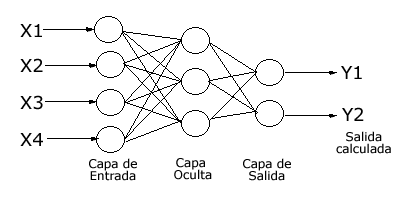
\includegraphics[width=0.4\linewidth]{images/perceptron_multicapa} 

}

\caption{Ejemplo de perceptrón multicapa}\label{fig:perceptron-multicapa}
\end{figure}

El problema habitual con este tipo de redes multicapa es el de, dados un
conjunto de datos ya clasificados, de los que se conoce la salida
deseada, proporcionar los pesos adecuados de la red para que se obtenga
una aproximación correcta de las salidas si la red recibe únicamente los
datos de entrada.

Estos sistemas aprenden y se forman a sí mismos, en lugar de ser
programados de forma explícita, y sobresalen en áreas donde la detección
de soluciones o características es difícil de expresar con la
programación convencional. Para realizar este aprendizaje automático,
normalmente, se intenta minimizar una \textbf{función de pérdida} que
evalúa la red en su total. Los valores de los pesos de las neuronas se
van actualizando buscando reducir el valor de la función de pérdida.
Este proceso se realiza mediante la \textbf{propagación hacia atrás}.

El objetivo de la red neuronal es resolver los problemas de la misma
manera que el cerebro humano, aunque las redes neuronales son más
abstractas. Las redes neuronales actuales suelen contener desde unos
miles a unos pocos millones de unidades neuronales.

Las redes neuronales se han utilizado para resolver una amplia variedad
de tareas, como la visión artificial y el reconocimiento de voz, que son
difíciles de resolver usando la ordinaria programación basada en reglas.
Históricamente, el uso de modelos de redes neuronales marcó un cambio de
dirección significativo a finales de los años ochenta. Se pasa de
sistemas expertos con conocimiento incorporado en reglas a sistemas
caracterizados por el conocimiento incorporado en los parámetros de un
modelo cognitivo.

Históricamente, el avance clave en el desarrollo de las redes neuronales
fue el \textbf{algoritmo de propagación hacia atrás} que resuelve
eficazmente el problema del entrenamiento rápido de redes neuronales de
múltiples capas \citep{werbos1975beyond}. El proceso de propagación
hacia atrás utiliza la diferencia entre el resultado producido y el
resultado deseado para cambiar los ``pesos'' de las conexiones entre las
neuronas artificiales.

Este algoritmo de entrenamiento de la red por propagación hacia atrás se
puede resumir muy brevemente en los siguiente puntos:

\begin{itemize}
\tightlist
\item
  Empezar con unos pesos sinápticos cualesquiera (generalmente elegidos
  al azar).
\item
  Introducir datos de entrada (en la capa de entrada) elegidos al azar
  entre el conjunto de datos de entrada que se van a usar para el
  entrenamiento.
\item
  Dejar que la red genere un vector de datos de salida (propagación
  hacia delante).
\item
  Comparar la salida generada por al red con la salida deseada.
\item
  La diferencia obtenida entre la salida generada y la deseada
  (denominada error) se usa para ajustar los pesos sinápticos de las
  neuronas de la capa de salidas.
\item
  El error se propaga hacia atrás (back-propagation), hacia la capa de
  neuronas anterior, y se usa para ajustar los pesos sinápticos en esta
  capa.
\item
  Se continúa propagando el error hacia atrás y ajustando los pesos
  hasta que se alcance la capa de entradas.
\item
  Este proceso se repetirá con los diferentes datos de entrenamiento.
\end{itemize}

Sin embargo, para redes de múltiples capas que usan la propagación hacia
atrás se presenta \textbf{el problema del desvanecimiento del
gradiente}. Un caso particular son las redes neuronales recurrentes
(RNNs). \textbf{Aunque los errores se propagan de una capa a otra,
disminuyen exponencialmente con el número de capas, y eso impide el
ajuste hacia atrás de los pesos de las neuronas basado en esos errores}.
Las redes profundas se ven particularmente afectadas. Más adelante
veremos cómo resolver este problema mediante el uso de unas redes
concretas.

\section{Estrategias de pronóstico}\label{estrategias-de-pronostico}

En los problemas con series temporales es muy común pronosticar más de
un valor en el futuro. En particular, esto es la parte central del
objetivo de este trabajo. Para este fin, se debe elegir una estrategia
de varios pasos adelante.

Esta cuestión suele abordarse de dos formas diferentes, que describimos
a continuación, pues utilizar una u otra ha sido del todo relevante en
los resultados arrojados por los métodos basados en redes neuronales.

\subsection{La estrategia de entrada múltiple y salida
múltiple}\label{la-estrategia-de-entrada-multiple-y-salida-multiple}

Esta estrategia se caracteriza por el uso de un vector de valores
objetivo. La longitud de este vector es igual a la cantidad de períodos
a pronosticar. Por ejemplo, pronosticar el flujo de tráfico para las
próximas 48 horas a intervalos de 15 minutos conlleva un vector objetivo
de \(48*4=192\) valores. La cantidad de valores pasados de la serie que
se consideren para pronosticar el vector objetivo es independiente del
tamaño del vector objetivo y dependerá en cada caso del algoritmo que se
utilice y de la naturaleza del problema.

En esta estrategia, una sóla ejecución del algoritmo, con los datos
pasados que necesite, da como resultado el pronóstico con el horizonte
necesario.

\subsection{La estrategia recursiva}\label{la-estrategia-recursiva}

La estrategia recursiva o iterativa es el enfoque utilizado, por
ejemplo, por ARIMA (método paramétrico, como vimos más arriba) para
pronosticar varios períodos. Básicamente, se utiliza un modelo que solo
pronostica un paso adelante, de modo que el modelo se aplica de forma
iterativa para pronosticar todos los períodos futuros. Cuando las
observaciones históricas que se usen como características de la nueva
instancia no estén disponibles, se pueden usar predicciones previas en
su lugar.

\section{Redes autorregresivas}\label{redes-autorregresivas}

Un primer acercamiento al uso de redes neuronales para el problema del
pronóstico del flujo de tráfico es utilizar las conocidas como redes
neuronales autorregresivas.

\begin{figure}[H]

{\centering 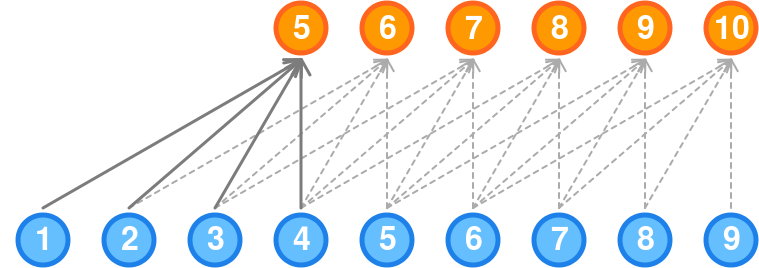
\includegraphics[width=0.4\linewidth]{images/nnar.simple} 

}

\caption{Arquitectura NNAR básica}\label{fig:NNAR-basic}
\end{figure}

La clave para el uso de este tipo de redes es considerar los datos
ordenados de la serie temporal como entradas de la red, del mismo modo
que usamos los valores retrasados en un modelo de autorregresión lineal.
A estos modelos se les llama redes neuronales de autorregresión o
modelos NNAR.

Cuando se trata de pronósticos utilizando este algoritmo, la red se
aplica de forma iterativa. Para pronosticar un paso adelante,
simplemente utilizamos las entradas históricas disponibles. Para
pronosticar dos pasos adelante, usamos el pronóstico de un paso como
entrada, junto con los datos históricos. Este proceso continúa hasta que
hayamos computado todos los pronósticos requeridos.

En lugar de implementar este tipo de redes desde cero, para los
experimentos que se han realizado en este trabajo se ha utilizado la
función \emph{nnetar} del paquete \emph{forecast} \citep{R-forecast}.

Sin embargo, los resultados obtenidos con este algoritmo para la batería
de experimentos realizados no han sido buenos. Aparte de lo negativo de
los resultados, los tiempos de cálculo son muy superiores a los
utilizados por otros algoritmos y métodos tratados. Esto motiva que el
presente estudio no haya seguido esta línea y que no se incluyan los
resultados en las tablas que se incluyen en los distintos apartados.

\section{LSTM univariado}\label{lstm-univariado}

Las redes neuronales recurrentes, RNN, son un tipo de redes capaces de
reconocer y predecir secuencias de datos a lo largo del tiempo, como
textos, genomas, discurso hablado o series numéricas. Este tipo de redes
se fundamentan en bucles que permiten que la salida de la red o de una
parte de ella en un momento dado sirva como entrada de la propia red en
el siguiente momento.

Para entender el funcionamiento de las RNNs, podemos considerar un
perceptrón multicapa con una sóla capa oculta de manera que la salida
del perceptrón es utilizada como entrada en la siguiente evaluación.
Este bucle en la arquitectura de la red es precisamente lo que permite a
la red ``recordar'' información a lo largo del tiempo. En la medida en
la que le añadimos capas, su capacidad de modelado irá creciendo de
manera que será capaz de reconocer mayores secuencias cada vez con menor
error.

\begin{figure}[H]

{\centering 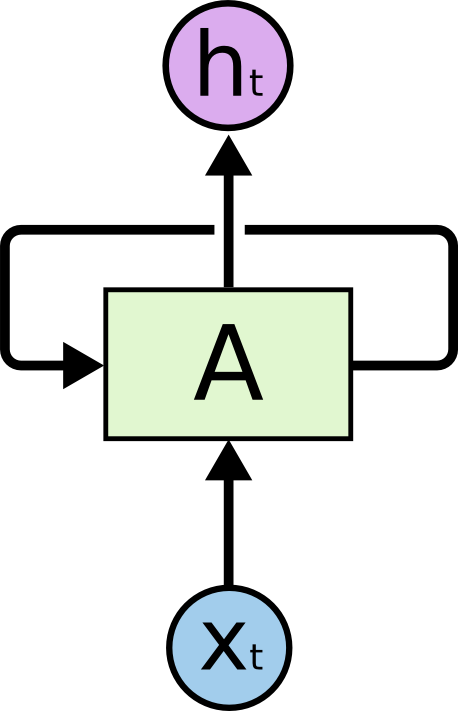
\includegraphics[width=0.1\linewidth]{images/RNN_basic} 

}

\caption{Arquitectura RNN básica}\label{fig:RNN-basic}
\end{figure}

Véase la Figura \ref{fig:RNN-basic}, dónde:

\begin{itemize}
\tightlist
\item
  \(\text{A}\) es una red neuronal
\item
  \(X_t\) es la entrada de la red
\item
  \(h_t\) es la salida de la red
\end{itemize}

Precisamente es el bucle que conecta la red consigo misma el mecanismo
que permite que la red tenga memoria.

Las RNNs pueden verse también como múltiples copias de la misma red,
cada una de ellas pasando información a su sucesora. Véase la Figura
\ref{fig:RNN-unrolled}. En cada momento del tiempo \(t\), la red recibe
como entrada tanto \(X_t\) como su propia salida \(h_{t-1}\) en el
instante \(t-1\).

\begin{figure}[H]

{\centering 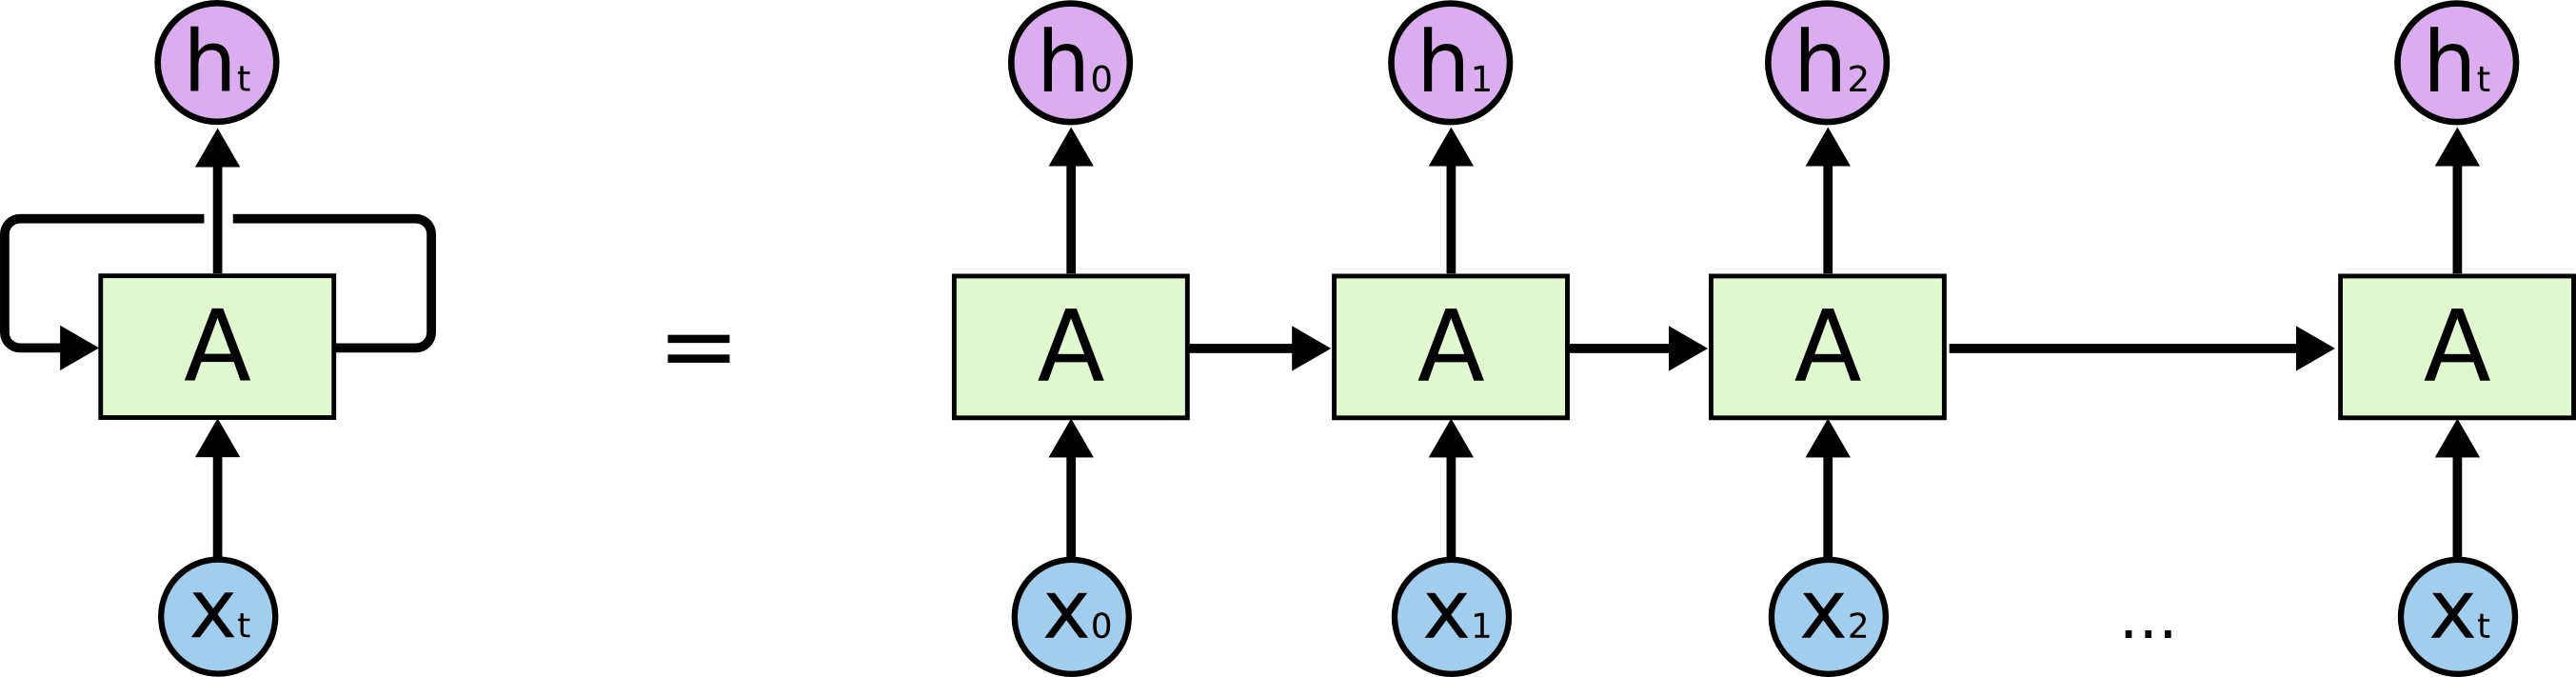
\includegraphics[width=0.6\linewidth]{images/RNN_unrolled} 

}

\caption{Arquitectura RNN expandida}\label{fig:RNN-unrolled}
\end{figure}

Las RNNs tienen un contratiempo importante conocido como
\textbf{problema del desvanecimiento del gradiente}; es decir, tienen
dificultades para aprender dependencias de largo alcance. Cuando se
realiza la propagación hacia atrás, es decir, nos movemos hacia atrás en
la red y calculamos los gradientes de pérdida (error) con respecto a los
pesos, los gradientes tienden a ser cada vez más pequeños a medida que
nos movemos hacia atrás en la red. Esto significa que las neuronas en
las capas anteriores aprenden muy lentamente en comparación con las
neuronas en las capas posteriores en la jerarquía. Las capas anteriores
de la red son las más lentas de entrenar. Este es un problema en todos
los tipos de redes neuronales, pero particularmente es nocivo para redes
en dónde lo que se pretende es tener la componente de memoria necesaria
para pronóstico de series temporales.

Afortunadamente, este problema fue resuelto por
\citep{hochreiter1997long} mediante la creación de las \textbf{LSTM}.
Las redes de memoria a corto/largo plazo, LSTM, son un tipo especial de
RNN, capaz de aprender dependencias a largo plazo.

Las LSTM están diseñados explícitamente para evitar el problema de
dependencia a largo plazo. Recordar información durante largos períodos
de tiempo es prácticamente su comportamiento predeterminado. Todas las
redes neuronales recurrentes tienen la forma de una cadena de módulos
repetitivos de la red neuronal. En las RNN estándar, este módulo de
repetición tendrá una estructura muy simple, como una sola capa de
activación. Los LSTM también tienen esta estructura tipo cadena, pero el
módulo de repetición tiene una estructura diferente. En lugar de tener
una sola capa de red neuronal, hay cuatro que interactúan de una manera
muy especial (Figura \ref{fig:LSTM-chain}).

\begin{figure}[H]

{\centering 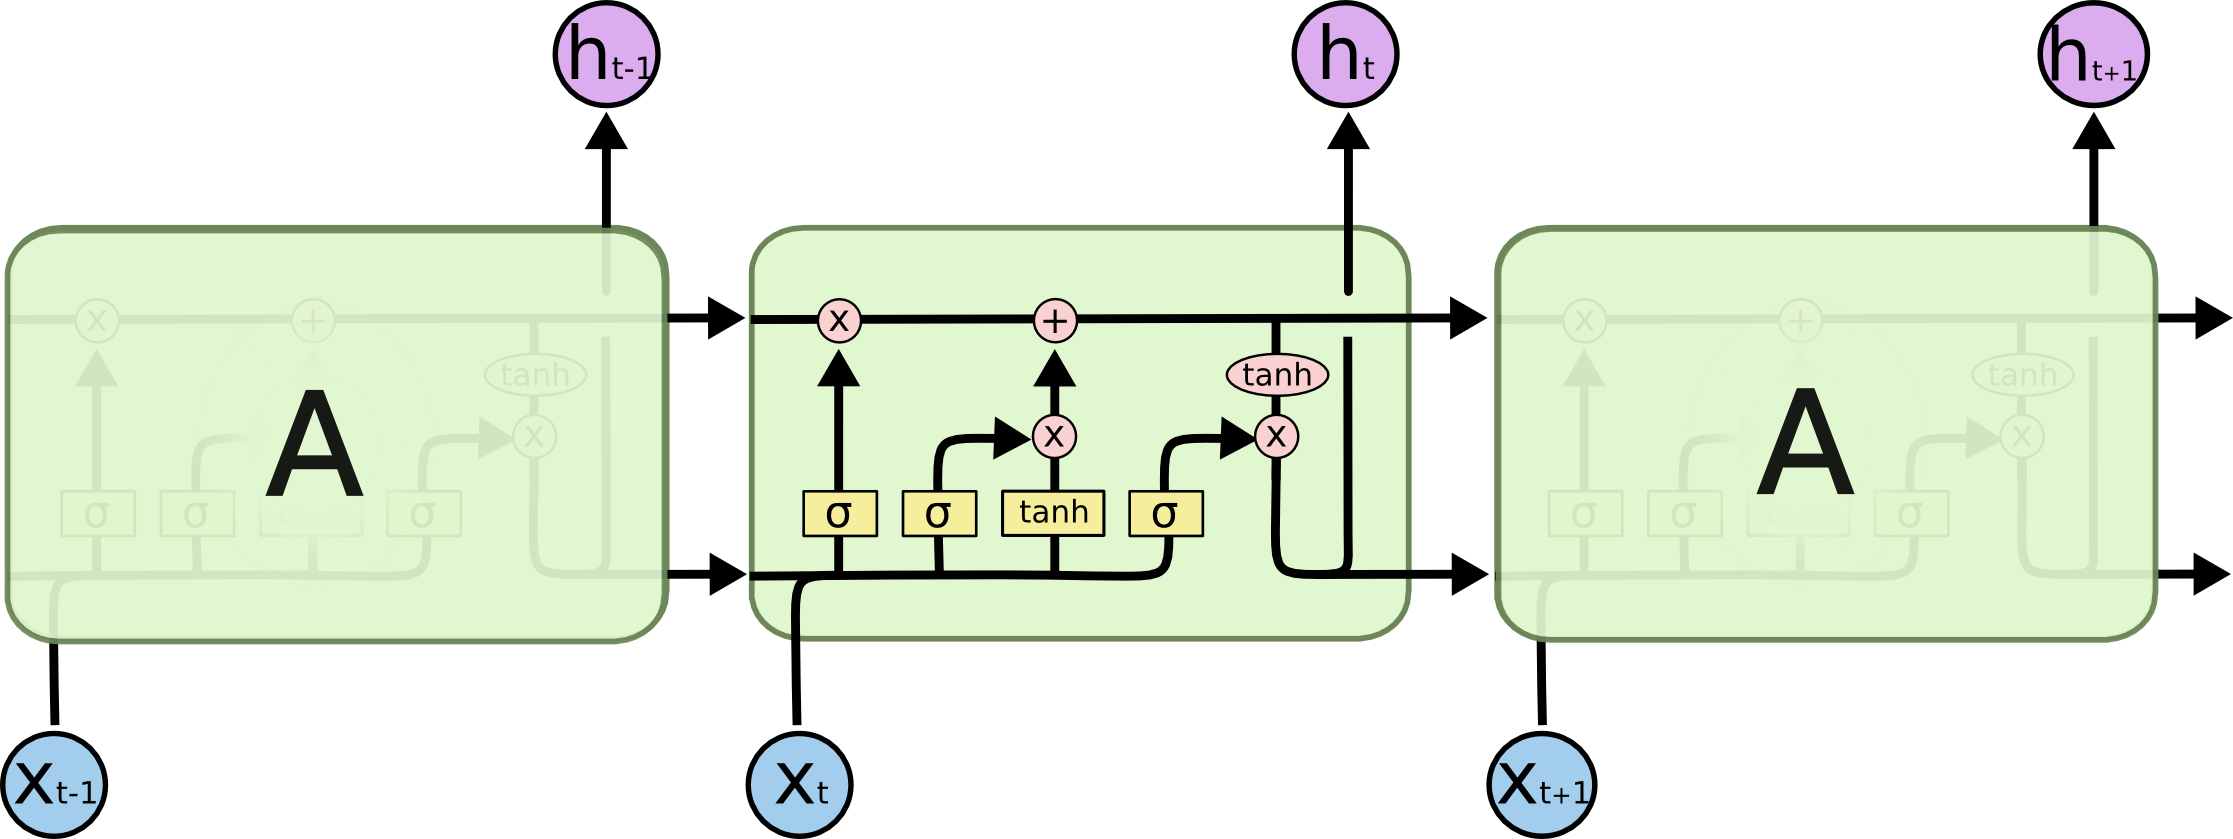
\includegraphics[width=0.6\linewidth]{images/LSTM3-chain} 

}

\caption{Capas de las celdas LSTM}\label{fig:LSTM-chain}
\end{figure}

La clave de las redes LSTM es el estado de la célula, la línea
horizontal que recorre la parte superior del diagrama. El estado de la
célula es algo así como una cinta transportadora. Corre hacia abajo por
toda la cadena, con solo algunas interacciones lineales menores. Es muy
fácil que la información fluya sin cambios. El LSTM tiene la capacidad
de eliminar o agregar información al estado de la célula, cuidadosamente
regulado por estructuras llamadas compuertas.

Las puertas son una forma de permitir que la información fluya. Se
componen de una capa de red neuronal sigmoidea y una operación de
multiplicación puntual. La capa sigmoide produce números entre cero y
uno, que describen la cantidad de cada componente que debe dejarse
pasar. Un valor de cero significa ``no dejar pasar nada'', mientras que
un valor de uno significa ``dejar pasar todo''. Un LSTM tiene tres de
estas compuertas, para proteger y controlar el estado de la celda.

Para ampliar conocimientos sobre el funcionamiento de las redes LSTM se
recomienda revisar el fantástico artículo \citep{olah2015lstm}.

Afortunadamente, para utilizar este tipo de red no es necesario
implementarlas desde cero, sino que se pueden utilizar distintos
frameworks. Como se explicará más adelante, los experimentos que hemos
realizado se han basado en Keras sobre TensorFlow.

\subsection{Descripción del
experimento}\label{descripcion-del-experimento}

Las LSTMs son sensibles a la escala de los datos de entrada,
especialmente cuando se utilizan las funciones de activación sigmoide
(por defecto) o tanh. Para evitar este problema, hemos reescalado los
datos al rango de 0 a 1.

La siguiente parte se relaciona con la estructura como se le presentan
las series a la red para que proceda al aprendizaje. Las redes LSTM, al
menos en la implementación de Keras, esperan una entrada del tipo
\emph{{[}muestras, pasos de tiempo, características{]}}. Para esto, dada
una serie de carga, se ha elegido un tamaño de sub-serie de
entrenamiento (\emph{look back}) y un tamaño de sub-serie de pronóstico
(\emph{look ahead}).

Sin embargo, es importante resaltar que en el caso de este algoritmo no
se han obtenido buenos resultados considerando la serie en crudo (con
los outlayers propios que pueda tener). Se ha comprobado que el
algoritmo converge mejor y da mejores resultados si la serie se suaviza
a granularidad de 1 hora.

En el contexto del suavizado indicado anteriormente, el valor \emph{look
ahead} utilizado es \(92/4 = 48\). Recordemos que el objetivo de esta
investigación son pronósticos a 48 horas vista (96 valores con
granularidad de 15 minutos, es decir, 48 con granularidad de una hora).

Respecto a la estrategia de pronóstico seguida, se ha utilizado la
múltiple. Se han realizado bastantes pruebas siguiendo la estrategia
recursiva no habiéndose llegado a resultados satisfactorios.

Tras muchas pruebas en las que se ha contrastado tanto los resultados
arrojados por el algoritmo como los recursos y tiempo necesarios para el
entrenamiento, se ha observado que un valor de \emph{look back} que
ofrece un buen rendimiento es tomar el mismo que se utiliza para
\emph{look ahead} (48 valores).

Por otro lado, hay dos formas de definir las redes LSTM en keras: redes
con estado (statefull) o redes sin estado (stateless) entre muestras
dentro del mismo lote de entrenamiento. Cuando se definen redes que con
estado, esto significa que las muestras que componen los diferentes
lotes de cada época de entrenamiento deben ser consecutivas en su índice
dentro del lote.

En este trabajo se han probado ambos enfoques no llegándose a conseguir
que las redes que no se definen con estado converjan.

Para las redes que se definen con estado, efectivamente sí se han
conseguido que converjan y los pronósticos, como veremos más adelante,
son relativamente satisfactorios. La parte que tiene que ver con
diseccionar una serie de carga en distintos lotes, garantizando que los
lotes satisfagan las indicaciones dadas más arriba ha sido realmente
trabajosa, pero finalmente los resultados han sido redes LSTM's capaces
de pronosticar el flujo.

Se ha prestado especial atención a que las redes no acaben
sobre-entrenadas. Esto se gestiona con bastante ergonomía en keras,
disponiendo de \emph{callbacks} que paran el entrenamiento cuando la
mejora en la disminución de errores no es significativa tras una o más
épocas.

En el capítulo de resultados veremos cómo se comportan estos algoritmos
en comparación con los métodos paramétricos que hemos explorado en los
apartados anteriores. Pero por ahora, por ejemplo, para el terminal
5575, en la Figura \ref{fig:LSTM-5575}, podemos ver los pronósticos
hechos con LSTM. Obsérvese como los pronósticos con LSTM están bastante
suavizados, en coherencia con los comentarios sobre suavizado de datos
hechos más arriba.

\begin{figure}[H]

{\centering \includegraphics[width=0.6\linewidth]{422.metodo.deep.lstm.univariado_files/figure-latex/LSTM-5575-1} 

}

\caption{Pronóstico del flujo de carga para el terminal 5.575 con LSTM}\label{fig:LSTM-5575}
\end{figure}

\section{LSTM con variables exógenas}\label{lstm-con-variables-exogenas}

En las series del flujo de tráfico existe una componente de
comportamiento humano que no debe ser despreciada. En particular, los
humanos ajustamos nuestros hábitos según las horas del día y los días de
la semana. Esta información viene reportada en los datos que hemos
trabajado, pero hasta ahora, en ninguno de los modelos anteriores hemos
considerado esta información como una variable de entrada.

Es de esperar que ayudando al modelo ofreciéndole como entrada esta
nueva fuente de información ofrezca un rendimiento mejor. En particular,
esto puede ser de especial utilidad en los modelos basados en
aprendizaje profundo, independientemente de que hay técnicas que
permiten seguir este enfoque también con los modelos paramétricos.

Esta técnica se ha seguido para algunos modelos basados en LSTM.
Concretamente, los modelos \textbf{LSTM-Exo DH Raw Scale Mean} y
\textbf{LSTM-Exo DH Agg5 Scale Mean} han sido construidos de este modo.

Para ambos modelos, se han utilizado además de los datos de carga de la
serie, dos nuevas \textbf{variables exógenas}, \emph{la hora del día} y
\emph{el día de la semana}. En lugar de construir modelos complejos, con
varias vías de entrada, se han encapsulado estas variables junto con la
carga en una única variable formada por 3 componentes. Como suele ser
habitual en el caso de redes neuronales, los datos han sido escalados al
intervalo {[}-1,1{]}.

En ambos casos, los resultados han mejorado bastante, como veremos en
detalle en el capítulo de resultados.

\chapter{Resultados}\label{resultados}

Uno de los objetivos fundamentales del presente trabajo es poner a
prueba distintos métodos y algoritmos de pronóstico de series temporales
para predecir el flujo de tráfico con los datos reportados por los
dispositivos de medida de la ciudad de Madrid.

Como hemos visto en los capítulos anteriores, se han utilizado métodos
paramétricos, basados en el modelado de series temporales
descomponiéndolas en componentes de tendencia y estacionalidad, métodos
basados en autorregresión y media móviles, y métodos basados en
aprendizaje profundo (deep learning).

Concretamente, se han puesto a prueba los métodos que pueden verse en la
siguiente lista. Para cada uno podemos ver una pequeña descripción de su
implementación. Para los detalles exactos del método, se recomienda
acudir al repositorio \citep{amanas-github}. Podemos ver que cada
experimento viene etiquetado con la familia de métodos a la que
pertenece. Esto nos permitirá más adelante seleccionar el mejor de cada
familia y expresar los resultados de una forma más clara o resumida
atendiendo sólo al método que mejor rinde por familia. Los métodos son:

\begin{itemize}
\tightlist
\item
  Familia ARIMA:

  \begin{itemize}
  \tightlist
  \item
    \textbf{AUTO ARIMA}. Método ARIMA ajustado automáticamente en cada
    serie.
  \item
    \textbf{SARIMA}. Método ARIMA estacional.
  \end{itemize}
\item
  Familia LSTM:

  \begin{itemize}
  \tightlist
  \item
    \textbf{LSTM Agg4 Diff}. LSTM entrenado con los datos de las 8
    semanas más recientes, transformando la serie a granularidad de una
    hora y diferenciando.
  \item
    \textbf{LSTM Agg4 Diff Scale Mean}. LSTM entrenado con los datos de
    las 8 semanas más recientes, transformando la serie a granularidad
    de una hora, diferenciando y escalando con centro y escala la media.
  \item
    \textbf{LSTM Agg4 Scale Mean}. LSTM entrenado con los datos de las 8
    semanas más recientes, transformando la serie a granularidad de una
    hora y escalando con centro y escala la media.
  \item
    \textbf{LSTM LSTM Agg4 Scale SD}. LSTM entrenado con los datos de
    las 8 semanas más recientes, transformando la serie a granularidad
    de una hora y escalando con centro la media y escala la desviación
    típica de la serie.
  \end{itemize}
\item
  Familia LSTM Exógeno:

  \begin{itemize}
  \tightlist
  \item
    \textbf{LSTM-Exo DH Agg5 Scale Mean}. LSTM entrenado con los datos
    de las 8 semanas más recientes, incorporando la hora del día y el
    día de la semana como variables exógenas, transformando la serie a
    granularidad de 75 minutos y escalando con centro y escala la media.
  \item
    \textbf{LSTM-Exo DH Raw Scale Mean}. LSTM entrenado con los datos de
    las 8 semanas más recientes, incorporando la hora del día y el día
    de la semana como variables exógenas y escalando con centro y escala
    la media.
  \end{itemize}
\item
  Familia MIXTO STL LSTM:

  \begin{itemize}
  \tightlist
  \item
    \textbf{STL+LSTM Agg5 Scale Mean}. Ajuste STL a 6 meses de datos más
    recientes de la serie considerando estacionalidad semanal.
    Posteriormente, los residuos de STL se modelan con LSTM
    transformando la serie a granularidad de 75 minutos.
  \item
    \textbf{STL+LSTM Raw Scale Mean}. Ajuste STL a 6 meses de datos más
    recientes de la serie considerando estacionalidad semanal.
    Posteriormente, los residuos de STL se modelan con LSTM
    transformando la serie a granularidad de 1 hora y escalando con
    centro y escala la media.
  \end{itemize}
\item
  Familia STL:

  \begin{itemize}
  \tightlist
  \item
    \textbf{STL D}. STL con estacionalidad diaria ajustado en toda la
    serie.
  \item
    \textbf{STL D Reciente}. STL con estacionalidad diaria ajustado en
    los 6 meses de datos previos al punto de pronóstico.
  \item
    \textbf{STL M}. STL con estacionalidad mensual ajustado en toda la
    serie.
  \item
    \textbf{STL M Reciente}. STL con estacionalidad mensual ajustado en
    los 6 meses de datos previos al punto de pronóstico.
  \item
    \textbf{STL W}. STL con estacionalidad semanal ajustado en toda la
    serie.
  \item
    \textbf{STL W Reciente}. STL con estacionalidad semanal ajustado en
    los 6 meses de datos previos al punto de pronóstico.
  \item
    \textbf{STL Y}. STL con estacionalidad anual ajustado en toda la
    serie.
  \end{itemize}
\item
  Familia STLM:

  \begin{itemize}
  \tightlist
  \item
    \textbf{STLM DW}. STLM con estacionalidades diaria y semanal
    ajustado en toda la serie.
  \item
    \textbf{STLM DWM}. STLM con estacionalidades diaria, semanal y
    mensual ajustado en toda la serie.
  \item
    \textbf{STLM DWM Reciente}. STLM con estacionalidades diaria,
    semanal y mensual ajustado en los 6 meses de datos previos al punto
    de pronóstico.
  \item
    \textbf{STLM DWY}. STLM con estacionalidades diaria, semanal y anual
    ajustado en toda la serie.
  \end{itemize}
\end{itemize}

La forma de realizar el experimento de contraste ha sido aplicar los
distintos algoritmos puestos a prueba a todas las series de tiempo y
comparar los resultados pronosticados por cada algoritmo contra la serie
conocida real. En número de dispositivos de los que se tienen datos
suficientes como para practicar estos experimentos es 3.976. Esto nos
permite confiar en que los promedios de error de cada algoritmo
realmente serán significativos de su capacidad de modelado y pronóstico.

Igualmente, el punto de prueba para cada serie se ha elegido
aleatoriamente en el intervalo de los últimos 12 meses de datos de la
serie, lo que nos libera de posibles sesgos que se pudieran producir por
seleccionar siempre puntos en un mismo día del año o de la semana o a
una misma hora del día. Recordemos, que como explicábamos más arriba,
todos los métodos aplicados a una serie se han aplicado sobre el mismo
instante aleatorio en los 12 meses más recientes. Pero este instante no
tiene por qué ser el mismo (y no lo es) para todas las series.

Cada algoritmo de los probados ofrece pronósticos a 48 horas vista con
una granularidad de 15 minutos. Esto nos permite someterlos a contraste
según diferentes horizontes de pronóstico. En el Cuadro
\ref{tab:exps-by-method-tab} podemos ver el número de experimentos
válidos realizados por cada método de los que citábamos en la lista de
anterior.

\begin{longtable}{llr}
\caption{\label{tab:exps-by-method-tab}Número de experimentos realizados por cada método}\\
\toprule
Familia & Nombre & Experimentos realizados\\
\midrule
\endfirsthead
\caption[]{\label{tab:exps-by-method-tab}Número de experimentos realizados por cada método \textit{(continued)}}\\
\toprule
Familia & Nombre & Experimentos realizados\\
\midrule
\endhead
\
\endfoot
\bottomrule
\endlastfoot
\rowcolor{gray!6}  ARIMA & AUTO ARIMA & 3975\\
ARIMA & SARIMA & 3970\\
\rowcolor{gray!6}  LSTM & LSTM Agg4 Diff & 3719\\
LSTM & LSTM Agg4 Diff Scale Mean & 3724\\
\rowcolor{gray!6}  LSTM & LSTM Agg4 Scale Mean & 3727\\
\addlinespace
LSTM & LSTM Agg4 Scale SD & 3725\\
\rowcolor{gray!6}  LSTM Exógeno & LSTM-Exo DH Agg5 Scale Mean & 3972\\
LSTM Exógeno & LSTM-Exo DH Raw Scale Mean & 3972\\
\rowcolor{gray!6}  MIXTO STL LSTM & STL+LSTM Agg5 Scale Mean & 2502\\
MIXTO STL LSTM & STL+LSTM Raw Scale Mean & 2508\\
\addlinespace
\rowcolor{gray!6}  STL & STL D & 3975\\
STL & STL D Reciente & 3975\\
\rowcolor{gray!6}  STL & STL M & 3973\\
STL & STL M Reciente & 3974\\
\rowcolor{gray!6}  STL & STL W & 3975\\
\addlinespace
STL & STL W Reciente & 3976\\
\rowcolor{gray!6}  STL & STL Y & 3704\\
STLM & STLM DW & 3976\\
\rowcolor{gray!6}  STLM & STLM DWM & 3976\\
STLM & STLM DWM Reciente & 3976\\
\addlinespace
\rowcolor{gray!6}  STLM & STLM DWY & 3976\\*
\end{longtable}

\textbf{En los próximos apartados, siempre que hablemos del error
cometido por cualquier método para un horizonte \(h\), nos referimos al
agregado de errores cometidos entre en el intervalo de predicciones que
van desde el primer valor pronosticado hasta el \(h\)-ésimo valor
pronosticado.} Es importante tener esto muy presente para la
interpretación de los resultados que veremos a continuación.

\section{Métricas de error}\label{metricas-de-error}

Un mismo pronóstico puede compararse con el valor real esperado
atendiendo a diferentes medidas de error.

Un ``error'' de pronóstico es la diferencia entre un valor observado y
su pronóstico. Es decir, ``error'' no significa un mal funcionamiento,
significa la parte impredecible de una observación. Se puede escribir
como:

\[e_T = y_T - \hat{y}_T\]

dónde \(\{ y_1, \dots, y_t \}, t \in T\), se refieren a los datos
observados y \(\{ \hat{y}_1, \dots, \hat{y}_t \}, t \in T\), son los
datos pronosticados.

A priori, no tiene por qué haber una medida del error que sea mejor que
otra; para cada caso, dependiendo de la naturaleza del fenómeno que se
pronostica, puede convenir utilizar unas u otras métricas, teniendo
siempre claro como interpretar la información arrojada por cada una.

Sin embargo, si conviene aclarar la diferencia que hay entre métricas
dependientes de la escala y métricas agnósticas de escala. Acudimos
nuevamente a \citep{Forecast6-online}.

\textbf{Las medidas de error dependientes de la escala} son aquellas en
las que las mediciones de los errores de pronóstico están en la misma
escala que los datos que se pronostican. El principal inconveniente de
este tipo de medida es que no se pueden usar para hacer comparaciones
entre series que involucran diferentes unidades o series que utilizando
la misma unidad tienen unos datos muy diferentes. Por ejemplo, si en una
vía la media de carga es del 50\% con una varianza del 50\% y en otra es
sólo del 2\% con una varianza del 5\%, si un método de pronóstico
tuviera un error \(\epsilon\) en ambas series, parece que podríamos
pensar que el método modela mejor la vía con mayor carga puesto que la
magnitud y variabilidad de los datos es mayor.

Las dos medidas dependientes de la escala más utilizadas se basan en los
errores absolutos (MAE) o los errores cuadrados (RMSE). Cuando se
comparan los métodos de pronóstico aplicados a una sola serie de tiempo,
o a varias series de tiempo con las mismas unidades, el MAE es popular
porque es fácil de entender y calcular. Un método de pronóstico que
minimiza el MAE conduce a pronósticos de la mediana, mientras que
minimizar el RMSE conduce a pronósticos de la media. En consecuencia, el
RMSE también se usa ampliamente, a pesar de ser más difícil de
interpretar. Más adelante veremos como se definen formalmente.

\textbf{Las medidas de error agnósticas de escala} típicamente se
expresan como porcentajes. Los errores de porcentaje tienen la ventaja
de estar libres de unidades, por lo que se usan con frecuencia para
comparar los rendimientos de pronóstico entre diferentes conjuntos de
datos. En el caso de nuestra investigación, esto es bastante importante
al ser bastante heterogéneo la distribución que adopta la carga según el
dispositivo (véanse las observaciones hechas más arriba sobre medidas
dependientes de la escala).

El porcentaje de error típicamente viene dado por:

\[p_t = 100 \frac{e_t}{y_t}, t \in T\]

siendo \(e_t\) el error cometido en el pronóstico en el instante \(t\),
\(y_{t}\) el valor real conocido.

La medida más utilizada es el MAPE, que definimos más adelante.

Las medidas basadas en errores de porcentaje tienen la desventaja de ser
infinitas o indefinidas si \(y_{t}=0\) para algún \(t\) en el período de
interés, y tener valores extremos si algún \(y_{t}\) está próximo a 0.

También tienen la desventaja de que imponen una mayor penalización a los
errores negativos que a los positivos. Esta observación condujo al uso
del llamado MAPE ``simétrico'' (sMAPE) propuesto por
\citep{armstrong1985long}, que no obstante, no utilizamos en nuestro
reporte.

Hechas las aclaraciones anteriores, que nos permitirán interpretar mejor
los resultados, describimos ahora cada una de las métricas utilizadas
\citep{hyndman2006another}:

\begin{itemize}
\tightlist
\item
  \textbf{ME (error medio)} es la media de los errores cometidos en el
  conjunto de pronósticos.
\end{itemize}

\[ ME = mean(e_t), t\in T \]

\begin{itemize}
\tightlist
\item
  \textbf{MAE (error absoluto medio)} es la media de los errores
  absolutos cometidos en el conjunto de pronósticos.
\end{itemize}

\[ MAE = mean(|e_t|), t\in T \]

\begin{itemize}
\tightlist
\item
  \textbf{RMSE (raiz del error cuadrático medio)} es la raíz cuadrada de
  la media de los errores cuadráticos cometidos en el conjunto de
  pronósticos.
\end{itemize}

\[ RMSE = \sqrt{\text{mean}(e_t^2)}, t\in T \]

\begin{itemize}
\tightlist
\item
  \textbf{MPE (error porcentual medio)} es la media de los errores
  porcentuales cometidos en el conjunto de pronósticos.
\end{itemize}

\[ MPE = mean(p_t), t\in T \]

\begin{itemize}
\tightlist
\item
  \textbf{MAPE (error porcentual absoluto medio)} es la media de los
  errores porcentuales absolutos cometidos en el conjunto de
  pronósticos.
\end{itemize}

\[ MAPE = mean(|p_t|), t\in T \]

\section{Mejores métodos por familia}\label{mejores-metodos-por-familia}

Tal como comentábamos en el apartado anterior, para una mejor exposición
de los resultados, sobre todo pensando en las gráficas, conviene en
primer lugar seleccionar el experimento que mejor rendimiento ha
ofrecido en el grupo o la familia a la que pertenece.

En ocasiones ocurre que dados dos métodos de los probados, aunque el
número de series en el que se han puesto a prueba es muy elevado
(cercano a la totalidad de las series que se estudian en este trabajo),
es posible que para una o varias series concretas sólo uno de los
métodos haya sido probado. Por eso, para la comparación de rendimientos
y selección del mejor método, siempre se considera el rendimiento en
aquellas series en las que todos los métodos han sido experimentados.

Conviene aclarar que, aunque se han registrado los 192 (2 días cada 15
minutos) pronósticos de cada método, para la presentación en cuadros de
los resultados sólo se utilizarán los pronósticos para horizontes de 1
hora vista, 4 horas vista, 12 horas vista, 24 horas vista y 48 horas
vista.

Veamos primero el método que mejor rendimiento ofrece en la familia
ARIMA. En el Cuadro \ref{tab:mejor-arima} vemos claramente que el mejor
rendimiento lo ofrece el método \textbf{SARIMA} (ARIMA estacional).

En el Cuadro \ref{tab:mejor-stl} revisamos los rendimientos para la
familia de métodos basada en la descomposición STL. Vemos claramente que
el mejor rendimiento lo ofrece el método \textbf{STL W Reciente} (STL
con estacionalidad semanal ajustado en los 6 meses de datos previos al
punto de pronóstico).

En el Cuadro \ref{tab:mejor-stlm} revisamos los rendimientos para la
familia de métodos basada en la descomposición STLM (STL considerando la
multiestacionalidad de las series). Vemos que el mejor rendimiento lo
ofrece el método \textbf{STLM DWM Reciente} (STLM con estacionalidades
diaria, semanal y mensual ajustado en los 6 meses de datos previos al
punto de pronóstico).

En el Cuadro \ref{tab:mejor-lstm} revisamos los rendimientos para la
familia de métodos basada en redes neuronales de tipo LSTM. Vemos que el
mejor rendimiento lo ofrece el método \textbf{LSTM Agg4 Scale SD} (LSTM
entrenado con los datos de las 8 semanas más recientes, transformando la
serie a granularidad de una hora y escalando con centro la media y
escala la desviación típica de la serie).

En el Cuadro \ref{tab:mejor-mixto} revisamos los rendimientos para la
familia de métodos MIXTO STL LSTM basada en redes neuronales de tipo
LSTM aplicadas a los residuos de utilizar STL. Vemos que los
rendimientos son muy similares aunque es sutilmente mejor el método
\textbf{STL+LSTM Agg5 Scale Mean} (Método mixto. Ajuste STL a 6 meses de
datos más recientes de la serie considerando estacionalidad semanal.
Posteriormente, los residuos de STL se modelan con LSTM transformando la
serie a granularidad de 75 minutos).

Y por último comprobamos los distintos experimentos realizados con redes
neuronales utilizando además variables exógenas. En el Cuadro
\ref{tab:mejor-exo} podemos ver que la diferencia no es muy grande pero
el mejor método es \textbf{LSTM-Exo DH Raw Scale Mean} (LSTM entrenado
con los datos de las 8 semanas más recientes, incorporando la hora del
día y el día de la semana como variables exógenas y escalando con centro
y escala la media).

\begin{table}[t]

\caption{\label{tab:mejor-arima}RMSE y MAPE para la familia de experimentos basados en ARIMA con horizonte de pronóstico a 1, 4, 12, 24 y 48 horas}
\centering
\resizebox{\linewidth}{!}{
\begin{tabular}{lrrrrrrrrrr}
\toprule
\multicolumn{1}{c}{ } & \multicolumn{5}{c}{RMSE} & \multicolumn{5}{c}{MAPE} \\
\cmidrule(l{3pt}r{3pt}){2-6} \cmidrule(l{3pt}r{3pt}){7-11}
Nombre & 1 horas & 4 horas & 12 horas & 24 horas & 48 horas & 1 horas & 4 horas & 12 horas & 24 horas & 48 horas\\
\midrule
\rowcolor{gray!6}  SARIMA & 3.97 & 5.64 & 7.04 & 7.67 & 8.17 & 32.1 & 39.27 & 44.89 & 49.64 & 49.69\\
AUTO ARIMA & 4.65 & 8.50 & 12.47 & 13.39 & 14.00 & 35.2 & 65.59 & 116.91 & 147.79 & 154.37\\
\bottomrule
\end{tabular}}
\end{table}

\begin{table}[t]

\caption{\label{tab:mejor-stl}RMSE y MAPE para la familia de experimentos basados en STL con horizonte de pronóstico a 1, 4, 12, 24 y 48 horas}
\centering
\resizebox{\linewidth}{!}{
\begin{tabular}{lrrrrrrrrrr}
\toprule
\multicolumn{1}{c}{ } & \multicolumn{5}{c}{RMSE} & \multicolumn{5}{c}{MAPE} \\
\cmidrule(l{3pt}r{3pt}){2-6} \cmidrule(l{3pt}r{3pt}){7-11}
Nombre & 1 horas & 4 horas & 12 horas & 24 horas & 48 horas & 1 horas & 4 horas & 12 horas & 24 horas & 48 horas\\
\midrule
\rowcolor{gray!6}  STL W Reciente & 3.65 & 5.04 & 6.53 & 6.87 & 7.18 & 27.44 & 33.76 & 45.87 & 52.11 & 52.43\\
STL W & 3.74 & 5.35 & 7.14 & 7.48 & 7.79 & 28.14 & 36.67 & 54.19 & 61.46 & 62.15\\
\rowcolor{gray!6}  STL D Reciente & 4.10 & 6.55 & 9.15 & 9.73 & 10.30 & 29.58 & 44.75 & 69.88 & 81.21 & 82.65\\
STL D & 4.15 & 6.73 & 9.54 & 10.15 & 10.69 & 29.87 & 46.05 & 73.99 & 86.43 & 87.50\\
\rowcolor{gray!6}  STL M & 4.82 & 9.37 & 16.43 & 17.68 & 18.15 & 32.92 & 62.12 & 142.87 & 174.87 & 177.34\\
\addlinespace
STL M Reciente & 5.53 & 10.35 & 17.81 & 19.23 & 19.64 & 48.18 & 78.52 & 163.75 & 199.73 & 200.74\\
\rowcolor{gray!6}  STL Y & 6.74 & 11.00 & 18.89 & 20.30 & 20.75 & 66.74 & 89.49 & 171.95 & 212.51 & 213.49\\
\bottomrule
\end{tabular}}
\end{table}

\begin{table}[t]

\caption{\label{tab:mejor-stlm}RMSE y MAPE para la familia de experimentos basados en STLM con horizonte de pronóstico a 1, 4, 12, 24 y 48 horas}
\centering
\resizebox{\linewidth}{!}{
\begin{tabular}{lrrrrrrrrrr}
\toprule
\multicolumn{1}{c}{ } & \multicolumn{5}{c}{RMSE} & \multicolumn{5}{c}{MAPE} \\
\cmidrule(l{3pt}r{3pt}){2-6} \cmidrule(l{3pt}r{3pt}){7-11}
Nombre & 1 horas & 4 horas & 12 horas & 24 horas & 48 horas & 1 horas & 4 horas & 12 horas & 24 horas & 48 horas\\
\midrule
\rowcolor{gray!6}  STLM DWM Reciente & 3.83 & 5.34 & 6.95 & 7.32 & 7.63 & 30.50 & 37.29 & 50.92 & 58.25 & 58.66\\
STLM DW & 3.73 & 5.32 & 7.10 & 7.45 & 7.76 & 28.07 & 36.36 & 53.44 & 60.68 & 61.30\\
\rowcolor{gray!6}  STLM DWM & 3.81 & 5.42 & 7.18 & 7.54 & 7.85 & 29.65 & 37.82 & 54.25 & 61.91 & 62.70\\
STLM DWY & 4.69 & 6.33 & 8.14 & 8.46 & 8.74 & 41.22 & 48.77 & 63.27 & 71.69 & 71.56\\
\bottomrule
\end{tabular}}
\end{table}

\begin{table}[t]

\caption{\label{tab:mejor-lstm}RMSE y MAPE para la familia de experimentos basados en LSTM con horizonte de pronóstico a 1, 4, 12, 24 y 48 horas}
\centering
\resizebox{\linewidth}{!}{
\begin{tabular}{lrrrrrrrrrr}
\toprule
\multicolumn{1}{c}{ } & \multicolumn{5}{c}{RMSE} & \multicolumn{5}{c}{MAPE} \\
\cmidrule(l{3pt}r{3pt}){2-6} \cmidrule(l{3pt}r{3pt}){7-11}
Nombre & 1 horas & 4 horas & 12 horas & 24 horas & 48 horas & 1 horas & 4 horas & 12 horas & 24 horas & 48 horas\\
\midrule
\rowcolor{gray!6}  LSTM Agg4 Scale SD & 5.77 & 6.34 & 7.18 & 7.81 & 8.45 & 43.52 & 42.30 & 45.57 & 48.92 & 50.28\\
LSTM Agg4 Scale Mean & 5.78 & 6.37 & 7.21 & 7.85 & 8.48 & 44.54 & 42.95 & 45.33 & 49.19 & 51.34\\
\rowcolor{gray!6}  LSTM Agg4 Diff Scale Mean & 4.50 & 7.12 & 9.59 & 10.75 & 12.48 & 29.90 & 44.29 & 64.77 & 79.61 & 90.12\\
LSTM Agg4 Diff & 4.60 & 7.52 & 10.74 & 12.01 & 14.12 & 29.76 & 45.29 & 69.19 & 86.81 & 99.52\\
\bottomrule
\end{tabular}}
\end{table}

\begin{table}[t]

\caption{\label{tab:mejor-mixto}RMSE y MAPE para la familia de experimentos basados en MIXTO con horizonte de pronóstico a 1, 4, 12, 24 y 48 horas}
\centering
\resizebox{\linewidth}{!}{
\begin{tabular}{lrrrrrrrrrr}
\toprule
\multicolumn{1}{c}{ } & \multicolumn{5}{c}{RMSE} & \multicolumn{5}{c}{MAPE} \\
\cmidrule(l{3pt}r{3pt}){2-6} \cmidrule(l{3pt}r{3pt}){7-11}
Nombre & 1 horas & 4 horas & 12 horas & 24 horas & 48 horas & 1 horas & 4 horas & 12 horas & 24 horas & 48 horas\\
\midrule
\rowcolor{gray!6}  STL+LSTM Agg5 Scale Mean & 4.37 & 5.32 & 6.31 & 6.57 & 6.92 & 34.91 & 36.83 & 45.53 & 49.12 & 48.75\\
STL+LSTM Raw Scale Mean & 3.72 & 4.89 & 6.39 & 6.68 & 7.02 & 26.45 & 31.57 & 45.65 & 50.00 & 49.69\\
\bottomrule
\end{tabular}}
\end{table}

\begin{table}[t]

\caption{\label{tab:mejor-exo}RMSE y MAPE para la familia de experimentos basados en LSTM Exógeno con horizonte de pronóstico a 1, 4, 12, 24 y 48 horas}
\centering
\resizebox{\linewidth}{!}{
\begin{tabular}{lrrrrrrrrrr}
\toprule
\multicolumn{1}{c}{ } & \multicolumn{5}{c}{RMSE} & \multicolumn{5}{c}{MAPE} \\
\cmidrule(l{3pt}r{3pt}){2-6} \cmidrule(l{3pt}r{3pt}){7-11}
Nombre & 1 horas & 4 horas & 12 horas & 24 horas & 48 horas & 1 horas & 4 horas & 12 horas & 24 horas & 48 horas\\
\midrule
\rowcolor{gray!6}  LSTM-Exo DH Raw Scale Mean & 5.15 & 5.56 & 6.08 & 6.35 & 6.85 & 36.91 & 34.21 & 34.47 & 35.04 & 35.80\\
LSTM-Exo DH Agg5 Scale Mean & 5.73 & 5.96 & 6.43 & 6.73 & 7.12 & 45.83 & 39.41 & 38.11 & 39.51 & 39.76\\
\bottomrule
\end{tabular}}
\end{table}

Por lo tanto, podemos recopilar las tablas de resultados anteriores
enumerando los mejores métodos por familias. Estos métodos serán los que
comparemos entre sí en los siguientes apartados. Son los que se enumeran
en el Cuadro \ref{tab:top-by-family}.

\begin{longtable}{ll}
\caption{\label{tab:top-by-family}Mejor método por familia}\\
\toprule
Familia & Método\\
\midrule
\endfirsthead
\caption[]{\label{tab:top-by-family}Mejor método por familia \textit{(continued)}}\\
\toprule
Familia & Método\\
\midrule
\endhead
\
\endfoot
\bottomrule
\endlastfoot
\rowcolor{gray!6}  ARIMA & SARIMA\\
LSTM & LSTM Agg4 Scale SD\\
\rowcolor{gray!6}  LSTM Exógeno & LSTM-Exo DH Raw Scale Mean\\
MIXTO STL LSTM & STL+LSTM Agg5 Scale Mean\\
\rowcolor{gray!6}  STL & STL W Reciente\\
\addlinespace
STLM & STLM DWM Reciente\\*
\end{longtable}

\newpage

\section{Comparación de resultados del mejor método por
familia}\label{comparacion-de-resultados-del-mejor-metodo-por-familia}

En el apartado anterior hemos visto cuál es el método que mejor rinde
por cada familia. En este apartado vamos a comparar los rendimiento de
esos mejores métodos y ver como se comparan unos con otros.

En primer estudiaremos los errores cometidos por los mejores métodos
teniendo en cuenta todas las series en las que han sido probados.
Recordemos que indicábamos más arriba que las series que se utilizan
para comparar el rendimiento de un conjunto de métodos son sólo aquellas
en las que todos los métodos del conjunto han sido probadas; de este
modo evitamos la influencia de cualquier tipo de sesgo que pudiera
ocurrir de que un método hubiera sido probado en series más convenientes
que otro.

En el Cuadro \ref{tab:accs-top-tab} podemos ver los errores cuadráticos
y absoluto medios cometidos por cada método de los seleccionados en el
punto anterior.

Podemos observar que en general, el método STL entrenado únicamente con
la cola reciente de los datos ofrece los mejores resultados para
horizontes pequeños (inferiores a 12 horas vista).

Sin embargo, para horizontes más grandes, vemos como el algoritmo LSTM
alimentado con variables exógenas mejora en los resultados. Esto se
aprecia principalmente en la métrica porcentual, en dónde no sólo se
tiene en cuenta el error que se comete sino como de grande es en
relación con el tamaño de la magnitud que se predice.

Por otro lado, en la Figura \ref{fig:accs-top-fig} se muestran los
distintos errores promedio cometidos por cada algoritmo, en este caso
calculados para todos los horizontes (desde 15 minutos hasta 48 horas).

\begin{table}[t]

\caption{\label{tab:accs-top-tab}RMSE y MAPE para el mejor método de cada familia con horizonte de pronóstico a 1, 4, 12, 24 y 48 horas}
\centering
\resizebox{\linewidth}{!}{
\begin{tabular}{lrrrrrrrrrr}
\toprule
\multicolumn{1}{c}{ } & \multicolumn{5}{c}{RMSE} & \multicolumn{5}{c}{MAPE} \\
\cmidrule(l{3pt}r{3pt}){2-6} \cmidrule(l{3pt}r{3pt}){7-11}
Nombre & 1 horas & 4 horas & 12 horas & 24 horas & 48 horas & 1 horas & 4 horas & 12 horas & 24 horas & 48 horas\\
\midrule
\rowcolor{gray!6}  LSTM-Exo DH Raw Scale Mean & 5.06 & 5.47 & 5.98 & 6.20 & 6.66 & 36.70 & 33.17 & 34.46 & 34.82 & 35.13\\
STL W Reciente & 3.63 & 4.86 & 6.20 & 6.57 & 6.88 & 28.18 & 33.23 & 43.29 & 49.60 & 49.54\\
\rowcolor{gray!6}  STL+LSTM Agg5 Scale Mean & 4.34 & 5.29 & 6.27 & 6.54 & 6.90 & 34.96 & 36.89 & 45.66 & 49.18 & 48.87\\
STLM DWM Reciente & 3.79 & 5.12 & 6.58 & 6.97 & 7.29 & 31.01 & 37.34 & 50.09 & 57.07 & 57.21\\
\rowcolor{gray!6}  SARIMA & 3.96 & 5.57 & 6.87 & 7.47 & 7.90 & 32.07 & 39.27 & 45.71 & 50.80 & 50.52\\
\addlinespace
LSTM Agg4 Scale SD & 5.51 & 6.09 & 6.95 & 7.56 & 8.16 & 40.21 & 39.50 & 45.07 & 48.24 & 49.14\\
\bottomrule
\end{tabular}}
\end{table}

\begin{figure}[H]

{\centering \includegraphics[width=1\linewidth]{503.resultados.todos_files/figure-latex/accs-top-fig-1} 

}

\caption{Gráfica de errores cometidos por los mejores métodos por familia para todos los horizontes}\label{fig:accs-top-fig}
\end{figure}

\textbf{Podemos observar que el método basado en LSTM utilizando como
variables exógenas la hora del día y el día de la semana, además de los
datos crudos de la serie escalados y centrados, es el que mejor
rendimiento ofrece en términos generales.} Sin embargo, en pronósticos a
muy corto plazo (inferiores a unas 6 horas) es el algoritmo ``STL W
Reciente'' el que mejor aproxima el pronóstico.

\section{Resultados segmentando por porcentaje de fallas en los
datos}\label{resultados-segmentando-por-porcentaje-de-fallas-en-los-datos}

Sin embargo, como vimos en el apartado de relativo a los datos, los
dispositivos no siempre reportan correctamente los datos. Es decir, hay
fallas en el reporte a lo largo del tiempo, que en algunos casos son
bastante significativas.

Para el correcto funcionamiento de los algoritmos es imperativo que la
serie no tenga fallas en los datos. Para sobreponerse a este problema,
en la mayoría de los casos se ha acudido a técnicas de interpolación
para reparar los datos faltantes. Es fácil comprender que este tipo de
técnicas pueden comprometer los resultados en la medida en la que el
modelo en cuestión se educa con datos ``ficticios'' que pueden
introducir sesgos.

Por eso, en el contraste de resultados, consideramos importante
distinguir la capacidad de pronóstico segmentando también por la calidad
de los datos reportados por los dispositivos.

Para proceder de este modo, filtramos las métricas obtenidas en los
puntos anteriores quedándonos sólo con aquellos experimentos que se ha
realizado sobre series que no superan ciertos umbrales de fallas y sobre
esto calculamos agregados de errores.

Podemos ver los resultados para series con porcentaje de fallas inferior
a 5\% en el Cuadro \ref{tab:accs-five-RMSE-MAPE} y en la Figura
\ref{fig:accs-five-RMSE-MAPE-fig}.

\begin{table}[t]

\caption{\label{tab:accs-five-RMSE-MAPE}RMSE y MAPE para el mejor método de cada familia evaluado en series con porcentaje de fallas en los datos inferior al 5\%}
\centering
\resizebox{\linewidth}{!}{
\begin{tabular}{lrrrrrrrrrr}
\toprule
\multicolumn{1}{c}{ } & \multicolumn{5}{c}{RMSE} & \multicolumn{5}{c}{MAPE} \\
\cmidrule(l{3pt}r{3pt}){2-6} \cmidrule(l{3pt}r{3pt}){7-11}
Nombre & 1 horas & 4 horas & 12 horas & 24 horas & 48 horas & 1 horas & 4 horas & 12 horas & 24 horas & 48 horas\\
\midrule
\rowcolor{gray!6}  STL+LSTM Agg5 Scale Mean & 4.39 & 5.21 & 6.22 & 6.53 & 6.86 & 29.91 & 30.11 & 41.67 & 42.92 & 42.77\\
LSTM-Exo DH Raw Scale Mean & 5.23 & 5.69 & 6.28 & 6.49 & 6.97 & 30.25 & 28.13 & 30.17 & 30.56 & 31.73\\
\rowcolor{gray!6}  STL W Reciente & 3.52 & 4.76 & 6.18 & 6.64 & 7.00 & 20.24 & 27.43 & 38.71 & 46.55 & 46.86\\
STLM DWM Reciente & 3.63 & 4.91 & 6.27 & 6.73 & 7.12 & 22.99 & 30.15 & 40.23 & 49.21 & 49.78\\
\rowcolor{gray!6}  LSTM Agg4 Scale SD & 5.99 & 6.28 & 7.33 & 8.09 & 8.86 & 37.25 & 33.41 & 41.26 & 45.92 & 49.66\\
\addlinespace
SARIMA & 3.91 & 5.99 & 7.71 & 8.66 & 9.13 & 23.42 & 37.98 & 47.17 & 56.47 & 52.84\\
\bottomrule
\end{tabular}}
\end{table}

\begin{figure}[H]

{\centering \includegraphics[width=1\linewidth]{504.resultados.segmentando_files/figure-latex/accs-five-RMSE-MAPE-fig-1} 

}

\caption{Gráfica de errores cometidos por los mejores métodos por familia evaluados en series con porcentaje de fallas inferior al 5\%}\label{fig:accs-five-RMSE-MAPE-fig}
\end{figure}

Podemos observar que nuevamente los resultados del algoritmo STL
considerando solo la subserie reciente son los mejores para pronósticos
cercanos en el tiempo. Siendo el método LSTM Exógeno el que brinda
mejores resultados para pronósticos más lejanos en el tiempo.

En la Figura \ref{fig:hist-errores} podemos ver la forma como se
distribuyen los errores cometidos por los mejores métodos por familia a
48 horas vista. Observamos como las distribuciones que presentan los
distintos métodos son bastante similares entre sí. Así mismo, al ser
distribuciones unimodales, no parece que haya ningún método que difiera
en comportamiento en diferentes conjuntos de series, más allá de la
calidad de los datos.

En relación a la calidad de los datos, vemos como los métodos diferentes
de SARIMA y LSTM Agg4 Scale SD, en sus predicciones a 48 horas vista, se
ven perjudicados cuando sólo se tienen en cuenta aquellas series con
escaso porcentaje de fallas. O visto de otro modo, el resto de métodos
distintos de estos dos parecen comportarse peor ante series con datos
deficientes.

\begin{figure}[H]

{\centering \includegraphics[width=1\linewidth]{504.resultados.segmentando_files/figure-latex/hist-errores-1} 

}

\caption{Distribución de los errores cometidos por método en pronósticos a 48 horas vista}\label{fig:hist-errores}
\end{figure}

\section{Reproductibilidad}\label{reproductibilidad}

Este trabajo y todos los experimentos en él descritos han sido
realizados de una u otra manera con el lenguaje de programación R y con
los distintos frameworks para creación de textos científicos que ofrece.
En particular, ha sido de gran utilidad la librería \emph{bookdown}
\citep{R-bookdown}. Todos los experimentos pueden reproducirse
ejecutando el código que se expone de manera pública en Github
\citep{amanas-github}.

Los datos descargados y procesados se han guardado en una base de datos
MySQL alojada en \href{https://aws.amazon.com/}{AWS} utilizando el
servicio de base de datos en la nube
\href{https://aws.amazon.com/es/rds/}{RDS}. Se ha guardado además el
detalle de todos los experimentos realizados, con las medidas de error
asociadas a cada experimento y la subserie pronosticada y esperada. Está
prevista la exposición de manera pública de los archivos que permitan
recrear la base de datos, facilitando así la continuidad de esta
investigación por quien estuviera interesado. Los ficheros se alojarán
en el servicio de almacenamiento masivo
\href{https://aws.amazon.com/es/s3/}{S3} de Amazon y la url pública de
acceso a los mismos se expondrá en el repositorio Github que
mencionábamos más arriba.

Finalmente, para la elaboración de este documento nos hemos servido de
tres proyectos con RStudio:

\begin{itemize}
\item
  Uno con las funciones de utilidad e implementaciones de los
  experimentos realizados.
\item
  Otro, a modo de espacio de trabajo para pruebas de concepto, dónde se
  han ido elaborando uno a uno los distintos apartados de este
  documento, a modo de \emph{Notebook de R} con \emph{Rmarkdown}
  \citep{R-rmarkdown}.
\item
  Y por último, un tercer proyecto en dónde se han ido consolidando los
  distintos apartados utilizando el framework \emph{bookdown}
  \citep{R-bookdown}.
\end{itemize}

Como decimos más arriba, todo este material quedará expuesto de manera
pública en \citep{amanas-github}. Durante el desarrollo del trabajo,
para dotarnos de privacidad, se han hospedado los repositorios de código
y documentos en \href{https://bitbucket.org}{Bitbucket}, también basado
en el sistema de control de versiones \href{https://git-scm.com/}{git}.

De suma importancia ha sido también la máquina
\href{http://ndowe.ia.uned.es:8787/}{ndowe} que la UNED pone a
disposición de sus alumnos como ayuda para el desarrollo de este tipo de
trabajos. La cantidad de computación que se ha necesitado para estos
experimentos hubiera supuesto un gasto prohibitivo en cualquier
proveedor de servicio en la nube y unos tiempos de ejecución enormes en
una máquina doméstica.

A modo de resumen:

\begin{itemize}
\item
  Se han utilizado más de 40 librerías del lenguaje R.
\item
  Se han realizado más de 280 commits de git (consolidaciones de
  código).
\item
  Se han generado más de 2.079 líneas de código para funciones de
  utilidad y ayuda.
\item
  Se ha necesitado de más de 2.000 horas de computación para la
  realización de los experimentos.
\end{itemize}

\chapter{Conclusiones}\label{conclusiones}

Nos planteábamos tres propósitos para la consecución de este trabajo:

\begin{itemize}
\item
  Recopilar los datos históricos del flujo de tráfico reportados por los
  dispositivos de medida de la ciudad de Madrid.
\item
  Analizarlos para determinar si pueden utilizarse para hacer
  pronósticos y determinar la propiedad más significativa de los mismos
  en términos de interpretabilidad.
\item
  Comparar sobre este conjunto de datos los nuevos métodos de modelado
  de series temporales basados en redes neuronales con los métodos
  paramétricos clásicos.
\end{itemize}

Efectivamente, aunque ha sido laborioso, los datos se han recopilado y
de su estudio se ha determinado que la propiedad que informa del
porcentaje de carga de la vía en un momento dado es significativa en sí
misma del estado de la vía y dispone de información suficiente como para
ser modelada por métodos de pronóstico (clásicos y basados en
aprendizaje profundo).

Hemos visto además que aunque los datos son muy amplios, suficientemente
como para contrastar el rendimiento de los distintos métodos sobre
ellos, en ocasiones (un porcentaje quizá demasiado elevado) padecen de
fallas que hacen que el problema de pronóstico acabe resultando más
complejo. No ha sido objeto de este estudio profundizar en las técnicas
de reparación de datos en series que padecen de secuencias de datos no
informados. Pero sí podemos decir que es un factor que dificulta el
trabajo. Por ello, en la sección de resultados se ha estudiado en dos
conjuntos: el de todas las series y el subconjunto de las series que
garantizan que el porcentaje de valores no informados sea menor del 5\%.
Se ha visto que en términos generales, aunque los resultados varían
sutilmente, las conclusiones son prácticamente las mismas.

\textbf{A muy corto plazo} (predicciones inferiores a unas 6 horas),
como hemos vistos en los cuadros y figuras de resultados, \textbf{los
métodos basados en el estudio de la tendencia y estacionalidad (sencilla
o múltiple, STL o STLM) brindan los mejores resultados}. Esto se ha
observado tanto si se consideran todas las series como si se consideran
sólo las que padecen de datos mal informados en porcentaje inferior al
5\%.

Sin embargo, \textbf{en los pronósticos a corto plazo} (inferiores a
unas 48 horas), \textbf{sí obtenemos resultados en dónde los métodos
basados en LSTM igualan e incluso superan a los modelos paramétricos}.

No podemos enunciar que ningún método basado en redes neuronales sea
significativamente mejor que los mejores métodos paramétricos probados.
Pero sí \textbf{resulta de gran satisfacción ver que al menos dos
métodos basados en LSTM si llegan a igualar y, aunque sutílmente, a
mejorar al mejor método paramétrico}. Esto deja una puerta abierta a
seguir con la investigación y la mejora de las técnicas basadas en redes
neuronales.

Por otra parte, es importante observar que según los resultados,
disponer de todos los datos de la serie no siempre ayuda a que el modelo
pronostique mejor. En particular, en todas las familias de modelos
probados se ha visto que el modelo con mejor rendimiento siempre ha sido
ajustado en los datos más recientes de la serie. Es decir, la
estacionalidad anual en este tipo de problema no parece que sea de gran
utilidad. Más bien parece que basta con observar los datos de los meses
más recientes al instante a partir del que se pronostica. De hecho, para
este tipo de series, este comportamiento parece que es algo común, según
se ha podido leer en varios de los documentos de referencia utilizados
para este trabajo.

\section{Trabajo futuro}\label{trabajo-futuro}

Como nota para posibles trabajos futuros, la impresión general es que
tal vez la investigación habría sido más sencilla descartando desde el
principio series con la información bastante perjudicada y haberse
centrado únicamente en aquellas con calidad superior a cierto umbral.

Por otro lado, también puede ser de utilidad en trabajos futuros tomar
una muestra de los dispositivos bastante representativa de la
heterogeneidad de las series y hacer los experimentos restringiéndose a
esta muestra. En este estudio, todos los experimentos se han realizado
sobre todas las series (salvo escasas excepciones) lo cual ha supuesto
una carga de computación y de tiempo muy elevada.

En relación con las redes neuronales, el diseño de modelos basados en
LSTM es bastante complejo. La arquitectura de la red viene determinada
por una gran cantidad de parámetros y los parámetros obedecen a
naturaleza e influencia muy diferente. Por ejemplo, se puede explorar el
espacio de parámetros atendiendo a múltiples factores:

\begin{enumerate}
\def\labelenumi{\arabic{enumi}.}
\item
  Longitud del histórico utilizado.
\item
  Variables exógenas.
\item
  Mayor o menor agregación de los datos de la serie.
\item
  La arquitectura de la entrada: modelos de entrada sencilla o múltiple.
\item
  La ventana de datos de entrada considerada en cada iteración de
  aprendizaje.
\item
  Las iteraciones de aprendizaje por época en modelos con estado (la
  secuencia de datos movida con la que se entrena el modelo).
\item
  La ventana de pronóstico, que puede ser el siguiente instante futuro e
  iterar la predicción retroalimentando con el resultado que va
  arrojando o pronosticar \emph{n} instantes futuros en una sola
  predicción, que ha sido el enfoque utilizado en este trabajo.
\item
  La transformación/normalización de los datos de entrada.
\item
  Etc.
\end{enumerate}

Como decimos, las posibilidades de investigación en el campo de redes
LSTM aplicadas al problema de pronóstico del flujo de tráfico son muy
variadas. Por desgracia, en el ámbito de este trabajo es imposible
abordar una tarea tan extensa y aquí solo presentamos unos resultados
que encontramos satisfactorios y que invitan a seguir esta vía de
investigacióń. Unos párrafos más arriba se indicaba la conveniencia de
centrar la investigación en un subconjunto de las series. En el caso de
LSTM, echando la vista atrás, sí entendemos que al menos en la parte de
prototipado y prueba de diferentes configuraciones, puede ser muy
conveniente realizar el trabajo con series de laboratorio.

De hecho, en el desarrollo de este trabajo para estos modelos ha sido
muy interesante el diseño de este tipo de series, controlando de
antemano los distintos patrones estacionales, e ir observando la
influencia de los distintos parámetros, arquitecturas y técnicas de
entrenamiento. Realmente deja un sabor agridulce tener que acotar el
ámbito de la investigación y no seguir con esta vía, que sí queda
abierta para futuras investigaciones.

Por otra parte, sería muy interesante la investigación de modelos
basados en LSTM pero alimentando con varias series el modelo. En el
ámbito de este trabajo no ha sido posible profundizar tanto en la
investigación, pero podría ser útil determinar la correlación que hay
entre los datos reportados por un dispositivo y los reportados por sus
vecinos. De esta manera, atendiendo a cierto grafo de influencias entre
los distintos dispositivos, se podría pensar en un clúster de modelos
LSTM multivariados. O incluso, y por qué no, un único modelo basado en
deep learning que admitan como entrada todas las series. Como decimos,
este tipo de experimentos ha excedido las posibilidades y recursos de
esta investigación, pues aquí ya sería necesaria una infraestructura de
cálculo de cierta dimensión.

Aunque lo hemos mencionado de pasada en el listado anterior, podría ser
muy conveniente investigar el rendimiento de redes en dónde las celdas
LSTM se alimenten con los datos de carga de la serie (con mayor o menor
transformación) y las variables exógeneas se alimentan por otras capas
del modelo. Estaríamos pensando aquí en un modelo de red mixta de doble
entrada, una rama para LSTM y otra para celdas ordinarias.

Pensando nuevamente en las redes neuronales, y aunque no se haya
experimentado en este trabajo, es de cierta abundancia la literatura en
la que se utilizan redes de convolución (típicamente utilizadas para el
reconocimiento de imágenes) también para problemas de pronóstico de
series temporales. Podría ser muy adecuado en el futuro realizar este
tipo de experimentos y ver si los resultados igualan o mejoran a los
aquí expuestos.

Y por último, en lo relativo a la utilidad del estudio, vemos que en
términos generales es posible modelar de manera bastante correcta las
diferentes series y que por lo tanto es factible dotarse de sistemas que
permitan realizar pronósticos para el estado de las diferentes vías de
la ciudad. Podría ser del todo factible pensar en un sistema que en
tiempo real proporcionara este tipo de información.

\bibliography{book.bib}


% \printindex


\end{document}
